\INEchaptercarta{Alumnos en diversificado}{}



\cajita{Inscritos en diversificado }{El número de  inscritos en diversificado, se obtiene a partir del total de los alumnos registrados al treinta de marzo de cada año escolar, que se inscriben en diversificado sin distinción de la edad
	
	 En el año 2009 se inscribieron 310,778 alumnos y en el año 2014 se inscribieron 396,461 alumnos, lo cual muestra un crecimiento de 27.6\%.}{Número de inscritos en el ciclo de educación diversificada}{República de Guatemala, serie histórica, en datos absolutos}{\ \\[0mm]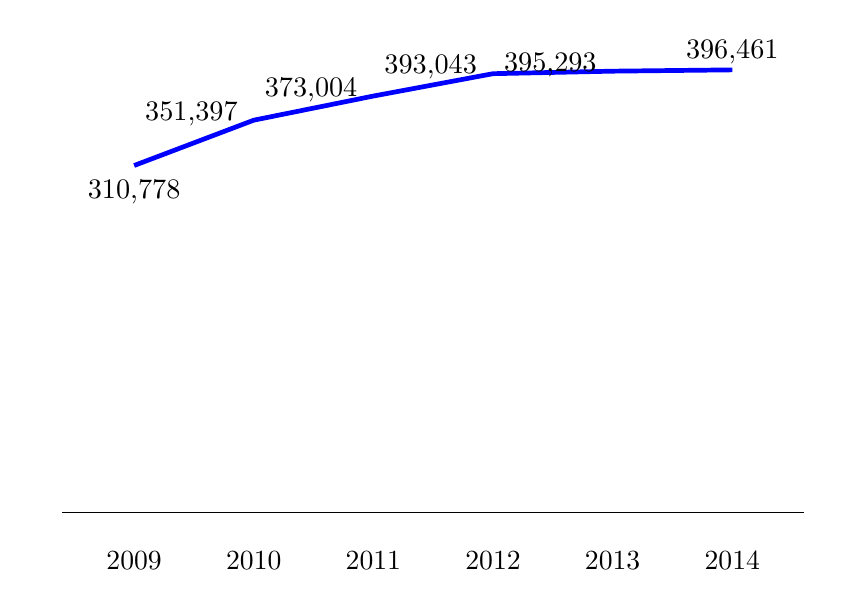
\begin{tikzpicture}[x=1pt,y=1pt]  % Created by tikzDevice version 0.10.1 on 2016-02-29 12:46:02
% !TEX encoding = UTF-8 Unicode
\definecolor{fillColor}{RGB}{255,255,255}
\path[use as bounding box,fill=fillColor,fill opacity=0.00] (0,0) rectangle (289.08,198.74);
\begin{scope}
\path[clip] (  0.00,  0.00) rectangle (289.08,198.74);

\path[] (  0.00,  0.00) rectangle (289.08,198.74);
\end{scope}
\begin{scope}
\path[clip] (  0.00,  0.00) rectangle (289.08,198.74);

\path[] ( 12.53, 15.61) rectangle (280.54,191.48);

\path[] ( 12.53, 43.75) --
	(280.54, 43.75);

\path[] ( 12.53, 84.08) --
	(280.54, 84.08);

\path[] ( 12.53,124.42) --
	(280.54,124.42);

\path[] ( 12.53,164.75) --
	(280.54,164.75);

\path[] ( 12.53, 23.58) --
	(280.54, 23.58);

\path[] ( 12.53, 63.92) --
	(280.54, 63.92);

\path[] ( 12.53,104.25) --
	(280.54,104.25);

\path[] ( 12.53,144.58) --
	(280.54,144.58);

\path[] ( 12.53,184.92) --
	(280.54,184.92);

\path[] ( 38.47, 15.61) --
	( 38.47,191.48);

\path[] ( 81.70, 15.61) --
	( 81.70,191.48);

\path[] (124.92, 15.61) --
	(124.92,191.48);

\path[] (168.15, 15.61) --
	(168.15,191.48);

\path[] (211.38, 15.61) --
	(211.38,191.48);

\path[] (254.61, 15.61) --
	(254.61,191.48);
\definecolor{drawColor}{RGB}{0,0,255}

\path[draw=drawColor,line width= 1.7pt,line join=round] ( 38.47,148.93) --
	( 81.70,165.31) --
	(124.92,174.03) --
	(168.15,182.11) --
	(211.38,183.02) --
	(254.61,183.49);
\definecolor{drawColor}{RGB}{0,0,0}

\node[text=drawColor,anchor=base,inner sep=0pt, outer sep=0pt, scale=  1.02] at ( 38.47,137.02) {310,778};

\node[text=drawColor,anchor=base east,inner sep=0pt, outer sep=0pt, scale=  1.02] at ( 75.90,165.31) {351,397};

\node[text=drawColor,anchor=base east,inner sep=0pt, outer sep=0pt, scale=  1.02] at (119.13,174.03) {373,004};

\node[text=drawColor,anchor=base east,inner sep=0pt, outer sep=0pt, scale=  1.02] at (162.35,182.11) {393,043};

\node[text=drawColor,anchor=base east,inner sep=0pt, outer sep=0pt, scale=  1.02] at (205.58,183.02) {395,293};

\node[text=drawColor,anchor=base,inner sep=0pt, outer sep=0pt, scale=  1.02] at (254.61,187.46) {396,461};

\path[draw=drawColor,line width= 0.1pt,line join=round] ( 12.53, 23.61) -- (280.54, 23.61);

\path[] ( 12.53, 15.61) rectangle (280.54,191.48);
\end{scope}
\begin{scope}
\path[clip] (  0.00,  0.00) rectangle (289.08,198.74);

\path[] ( 12.53, 15.61) --
	( 12.53,191.48);
\end{scope}
\begin{scope}
\path[clip] (  0.00,  0.00) rectangle (289.08,198.74);
\definecolor{drawColor}{RGB}{255,255,255}

\node[text=drawColor,text opacity=0.00,anchor=base east,inner sep=0pt, outer sep=0pt, scale=  1.00] at (  7.58, 19.67) {0e+00};

\node[text=drawColor,text opacity=0.00,anchor=base east,inner sep=0pt, outer sep=0pt, scale=  1.00] at (  7.58, 60.01) {1e+05};

\node[text=drawColor,text opacity=0.00,anchor=base east,inner sep=0pt, outer sep=0pt, scale=  1.00] at (  7.58,100.34) {2e+05};

\node[text=drawColor,text opacity=0.00,anchor=base east,inner sep=0pt, outer sep=0pt, scale=  1.00] at (  7.58,140.67) {3e+05};

\node[text=drawColor,text opacity=0.00,anchor=base east,inner sep=0pt, outer sep=0pt, scale=  1.00] at (  7.58,181.01) {4e+05};
\end{scope}
\begin{scope}
\path[clip] (  0.00,  0.00) rectangle (289.08,198.74);

\path[] (  9.78, 23.58) --
	( 12.53, 23.58);

\path[] (  9.78, 63.92) --
	( 12.53, 63.92);

\path[] (  9.78,104.25) --
	( 12.53,104.25);

\path[] (  9.78,144.58) --
	( 12.53,144.58);

\path[] (  9.78,184.92) --
	( 12.53,184.92);
\end{scope}
\begin{scope}
\path[clip] (  0.00,  0.00) rectangle (289.08,198.74);

\path[] ( 12.53, 15.61) --
	(280.54, 15.61);
\end{scope}
\begin{scope}
\path[clip] (  0.00,  0.00) rectangle (289.08,198.74);

\path[] ( 38.47, 12.86) --
	( 38.47, 15.61);

\path[] ( 81.70, 12.86) --
	( 81.70, 15.61);

\path[] (124.92, 12.86) --
	(124.92, 15.61);

\path[] (168.15, 12.86) --
	(168.15, 15.61);

\path[] (211.38, 12.86) --
	(211.38, 15.61);

\path[] (254.61, 12.86) --
	(254.61, 15.61);
\end{scope}
\begin{scope}
\path[clip] (  0.00,  0.00) rectangle (289.08,198.74);
\definecolor{drawColor}{RGB}{0,0,0}

\node[text=drawColor,anchor=base,inner sep=0pt, outer sep=0pt, scale=  1.00] at ( 38.47,  2.85) {2009};

\node[text=drawColor,anchor=base,inner sep=0pt, outer sep=0pt, scale=  1.00] at ( 81.70,  2.85) {2010};

\node[text=drawColor,anchor=base,inner sep=0pt, outer sep=0pt, scale=  1.00] at (124.92,  2.85) {2011};

\node[text=drawColor,anchor=base,inner sep=0pt, outer sep=0pt, scale=  1.00] at (168.15,  2.85) {2012};

\node[text=drawColor,anchor=base,inner sep=0pt, outer sep=0pt, scale=  1.00] at (211.38,  2.85) {2013};

\node[text=drawColor,anchor=base,inner sep=0pt, outer sep=0pt, scale=  1.00] at (254.61,  2.85) {2014};
\end{scope}
  \end{tikzpicture}}{Instituto Nacional de Estadística, con datos del Ministerio de Educación}

\cajita{Inscritos en diversificado por sexo}{En la gráfica  se observa que el porcentaje de hombres inscritos en diversificado fue del 49.9\% y de mujeres 50.1\%.}{Distribución de inscritos en el ciclo de\\ educación diversificada, por sexo}{República de Guatemala, año 2014, en porcentaje}{\ \\[0mm]\begin{tikzpicture}[x=1pt,y=1pt]  % Created by tikzDevice version 0.10.1 on 2016-02-29 12:46:26
% !TEX encoding = UTF-8 Unicode
\definecolor{fillColor}{RGB}{255,255,255}
\path[use as bounding box,fill=fillColor,fill opacity=0.00] (0,0) rectangle (289.08,198.74);
\begin{scope}
\path[clip] ( 30.54,  0.00) rectangle (258.54,198.74);

\path[] ( 30.54,  0.00) rectangle (258.54,198.74);
\end{scope}
\begin{scope}
\path[clip] (  0.00,  0.00) rectangle (289.08,198.74);

\path[] (  7.11,  4.95) rectangle (200.91,198.74);

\path[] (104.01,101.85) --
	(191.22,101.49);

\path[] (104.01,101.85) --
	( 16.80,102.21);

\path[] (104.01,101.85) --
	(104.37,189.05);

\path[] (104.01,101.85) --
	(191.22,101.49);

\path[] (104.01,101.85) --
	(103.65, 14.64);

\path[] (104.01,101.85) --
	( 16.80,102.21);

\path[] (104.01,101.85) --
	(104.01,101.85) --
	(104.01,101.85) --
	(104.01,101.85) --
	(104.01,101.85) --
	(104.01,101.85) --
	(104.01,101.85) --
	(104.01,101.85) --
	(104.01,101.85) --
	(104.01,101.85) --
	(104.01,101.85) --
	(104.01,101.85) --
	(104.01,101.85) --
	(104.01,101.85) --
	(104.01,101.85) --
	(104.01,101.85) --
	(104.01,101.85) --
	(104.01,101.85) --
	(104.01,101.85) --
	(104.01,101.85) --
	(104.01,101.85) --
	(104.01,101.85) --
	(104.01,101.85) --
	(104.01,101.85) --
	(104.01,101.85) --
	(104.01,101.85) --
	(104.01,101.85) --
	(104.01,101.85) --
	(104.01,101.85) --
	(104.01,101.85) --
	(104.01,101.85) --
	(104.01,101.85) --
	(104.01,101.85) --
	(104.01,101.85) --
	(104.01,101.85) --
	(104.01,101.85) --
	(104.01,101.85) --
	(104.01,101.85) --
	(104.01,101.85) --
	(104.01,101.85) --
	(104.01,101.85) --
	(104.01,101.85) --
	(104.01,101.85) --
	(104.01,101.85) --
	(104.01,101.85) --
	(104.01,101.85) --
	(104.01,101.85) --
	(104.01,101.85) --
	(104.01,101.85) --
	(104.01,101.85) --
	(104.01,101.85) --
	(104.01,101.85) --
	(104.01,101.85) --
	(104.01,101.85) --
	(104.01,101.85) --
	(104.01,101.85) --
	(104.01,101.85) --
	(104.01,101.85) --
	(104.01,101.85) --
	(104.01,101.85) --
	(104.01,101.85) --
	(104.01,101.85) --
	(104.01,101.85) --
	(104.01,101.85) --
	(104.01,101.85) --
	(104.01,101.85) --
	(104.01,101.85) --
	(104.01,101.85) --
	(104.01,101.85) --
	(104.01,101.85) --
	(104.01,101.85) --
	(104.01,101.85) --
	(104.01,101.85) --
	(104.01,101.85) --
	(104.01,101.85) --
	(104.01,101.85) --
	(104.01,101.85) --
	(104.01,101.85) --
	(104.01,101.85) --
	(104.01,101.85) --
	(104.01,101.85) --
	(104.01,101.85) --
	(104.01,101.85) --
	(104.01,101.85) --
	(104.01,101.85) --
	(104.01,101.85) --
	(104.01,101.85) --
	(104.01,101.85) --
	(104.01,101.85) --
	(104.01,101.85) --
	(104.01,101.85) --
	(104.01,101.85) --
	(104.01,101.85) --
	(104.01,101.85) --
	(104.01,101.85) --
	(104.01,101.85) --
	(104.01,101.85) --
	(104.01,101.85) --
	(104.01,101.85) --
	(104.01,101.85);

\path[] (104.01,121.23) --
	(105.24,121.19) --
	(106.46,121.07) --
	(107.68,120.88) --
	(108.88,120.60) --
	(110.06,120.26) --
	(111.21,119.84) --
	(112.34,119.34) --
	(113.43,118.78) --
	(114.49,118.15) --
	(115.50,117.45) --
	(116.47,116.69) --
	(117.38,115.87) --
	(118.25,115.00) --
	(119.05,114.07) --
	(119.80,113.09) --
	(120.48,112.06) --
	(121.09,111.00) --
	(121.64,109.90) --
	(122.11,108.76) --
	(122.51,107.60) --
	(122.84,106.42) --
	(123.09,105.21) --
	(123.27,103.99) --
	(123.37,102.77) --
	(123.39,101.54) --
	(123.33,100.31) --
	(123.19, 99.09) --
	(122.98, 97.88) --
	(122.69, 96.68) --
	(122.32, 95.51) --
	(121.88, 94.36) --
	(121.37, 93.24) --
	(120.79, 92.16) --
	(120.14, 91.11) --
	(119.43, 90.11) --
	(118.66, 89.16) --
	(117.82, 88.25) --
	(116.93, 87.40) --
	(115.99, 86.61) --
	(115.00, 85.88) --
	(113.96, 85.22) --
	(112.89, 84.62) --
	(111.78, 84.09) --
	(110.64, 83.64) --
	(109.47, 83.25) --
	(108.28, 82.94) --
	(107.07, 82.71) --
	(105.85, 82.55) --
	(104.62, 82.48) --
	(103.39, 82.48) --
	(102.17, 82.55) --
	(100.95, 82.71) --
	( 99.74, 82.94) --
	( 98.55, 83.25) --
	( 97.38, 83.64) --
	( 96.24, 84.09) --
	( 95.13, 84.62) --
	( 94.05, 85.22) --
	( 93.02, 85.88) --
	( 92.03, 86.61) --
	( 91.09, 87.40) --
	( 90.20, 88.25) --
	( 89.36, 89.16) --
	( 88.59, 90.11) --
	( 87.87, 91.11) --
	( 87.23, 92.16) --
	( 86.65, 93.24) --
	( 86.13, 94.36) --
	( 85.70, 95.51) --
	( 85.33, 96.68) --
	( 85.04, 97.88) --
	( 84.83, 99.09) --
	( 84.69,100.31) --
	( 84.63,101.54) --
	( 84.65,102.77) --
	( 84.75,103.99) --
	( 84.92,105.21) --
	( 85.18,106.42) --
	( 85.50,107.60) --
	( 85.91,108.76) --
	( 86.38,109.90) --
	( 86.93,111.00) --
	( 87.54,112.06) --
	( 88.22,113.09) --
	( 88.97,114.07) --
	( 89.77,115.00) --
	( 90.64,115.87) --
	( 91.55,116.69) --
	( 92.52,117.45) --
	( 93.53,118.15) --
	( 94.59,118.78) --
	( 95.68,119.34) --
	( 96.81,119.84) --
	( 97.96,120.26) --
	( 99.14,120.60) --
	(100.34,120.88) --
	(101.56,121.07) --
	(102.78,121.19) --
	(104.01,121.23);

\path[] (104.01,140.60) --
	(106.47,140.53) --
	(108.92,140.29) --
	(111.34,139.90) --
	(113.74,139.36) --
	(116.10,138.67) --
	(118.41,137.83) --
	(120.67,136.84) --
	(122.85,135.72) --
	(124.96,134.45) --
	(126.99,133.06) --
	(128.92,131.54) --
	(130.76,129.90) --
	(132.48,128.14) --
	(134.09,126.29) --
	(135.58,124.33) --
	(136.94,122.28) --
	(138.17,120.15) --
	(139.27,117.95) --
	(140.22,115.68) --
	(141.02,113.35) --
	(141.68,110.98) --
	(142.18,108.58) --
	(142.53,106.14) --
	(142.72,103.69) --
	(142.76,101.23) --
	(142.65, 98.77) --
	(142.37, 96.33) --
	(141.95, 93.91) --
	(141.37, 91.52) --
	(140.64, 89.17) --
	(139.76, 86.87) --
	(138.74, 84.63) --
	(137.58, 82.47) --
	(136.28, 80.38) --
	(134.85, 78.37) --
	(133.30, 76.46) --
	(131.63, 74.66) --
	(129.85, 72.96) --
	(127.97, 71.38) --
	(125.99, 69.92) --
	(123.92, 68.59) --
	(121.77, 67.40) --
	(119.55, 66.34) --
	(117.27, 65.43) --
	(114.93, 64.66) --
	(112.55, 64.04) --
	(110.13, 63.57) --
	(107.69, 63.26) --
	(105.24, 63.11) --
	(102.78, 63.11) --
	(100.33, 63.26) --
	( 97.89, 63.57) --
	( 95.47, 64.04) --
	( 93.09, 64.66) --
	( 90.75, 65.43) --
	( 88.47, 66.34) --
	( 86.25, 67.40) --
	( 84.10, 68.59) --
	( 82.03, 69.92) --
	( 80.05, 71.38) --
	( 78.17, 72.96) --
	( 76.39, 74.66) --
	( 74.72, 76.46) --
	( 73.17, 78.37) --
	( 71.74, 80.38) --
	( 70.44, 82.47) --
	( 69.28, 84.63) --
	( 68.26, 86.87) --
	( 67.38, 89.17) --
	( 66.65, 91.52) --
	( 66.07, 93.91) --
	( 65.65, 96.33) --
	( 65.37, 98.77) --
	( 65.26,101.23) --
	( 65.29,103.69) --
	( 65.49,106.14) --
	( 65.84,108.58) --
	( 66.34,110.98) --
	( 67.00,113.35) --
	( 67.80,115.68) --
	( 68.75,117.95) --
	( 69.85,120.15) --
	( 71.08,122.28) --
	( 72.44,124.33) --
	( 73.93,126.29) --
	( 75.54,128.14) --
	( 77.26,129.90) --
	( 79.10,131.54) --
	( 81.03,133.06) --
	( 83.06,134.45) --
	( 85.17,135.72) --
	( 87.35,136.84) --
	( 89.60,137.83) --
	( 91.92,138.67) --
	( 94.28,139.36) --
	( 96.67,139.90) --
	( 99.10,140.29) --
	(101.55,140.53) --
	(104.01,140.60);

\path[] (104.01,159.98) --
	(107.70,159.87) --
	(111.37,159.52) --
	(115.01,158.93) --
	(118.61,158.12) --
	(122.15,157.08) --
	(125.62,155.82) --
	(129.00,154.34) --
	(132.28,152.65) --
	(135.44,150.75) --
	(138.48,148.66) --
	(141.38,146.38) --
	(144.13,143.92) --
	(146.72,141.29) --
	(149.13,138.51) --
	(151.37,135.57) --
	(153.41,132.50) --
	(155.26,129.30) --
	(156.89,126.00) --
	(158.32,122.59) --
	(159.53,119.11) --
	(160.51,115.55) --
	(161.26,111.94) --
	(161.79,108.29) --
	(162.08,104.61) --
	(162.14,100.92) --
	(161.96, 97.24) --
	(161.56, 93.57) --
	(160.91, 89.94) --
	(160.05, 86.35) --
	(158.95, 82.83) --
	(157.63, 79.39) --
	(156.10, 76.03) --
	(154.36, 72.78) --
	(152.41, 69.64) --
	(150.27, 66.64) --
	(147.95, 63.77) --
	(145.44, 61.06) --
	(142.77, 58.52) --
	(139.95, 56.15) --
	(136.98, 53.96) --
	(133.87, 51.97) --
	(130.65, 50.17) --
	(127.32, 48.59) --
	(123.89, 47.21) --
	(120.39, 46.06) --
	(116.82, 45.14) --
	(113.20, 44.44) --
	(109.54, 43.97) --
	(105.85, 43.74) --
	(102.16, 43.74) --
	( 98.48, 43.97) --
	( 94.82, 44.44) --
	( 91.20, 45.14) --
	( 87.63, 46.06) --
	( 84.13, 47.21) --
	( 80.70, 48.59) --
	( 77.37, 50.17) --
	( 74.15, 51.97) --
	( 71.04, 53.96) --
	( 68.07, 56.15) --
	( 65.25, 58.52) --
	( 62.58, 61.06) --
	( 60.07, 63.77) --
	( 57.75, 66.64) --
	( 55.61, 69.64) --
	( 53.66, 72.78) --
	( 51.92, 76.03) --
	( 50.39, 79.39) --
	( 49.07, 82.83) --
	( 47.97, 86.35) --
	( 47.10, 89.94) --
	( 46.46, 93.57) --
	( 46.05, 97.24) --
	( 45.88,100.92) --
	( 45.94,104.61) --
	( 46.23,108.29) --
	( 46.75,111.94) --
	( 47.51,115.55) --
	( 48.49,119.11) --
	( 49.70,122.59) --
	( 51.13,126.00) --
	( 52.76,129.30) --
	( 54.61,132.50) --
	( 56.65,135.57) --
	( 58.89,138.51) --
	( 61.30,141.29) --
	( 63.89,143.92) --
	( 66.64,146.38) --
	( 69.54,148.66) --
	( 72.58,150.75) --
	( 75.74,152.65) --
	( 79.02,154.34) --
	( 82.40,155.82) --
	( 85.87,157.08) --
	( 89.41,158.12) --
	( 93.01,158.93) --
	( 96.65,159.52) --
	(100.32,159.87) --
	(104.01,159.98);

\path[] (104.01,179.36) --
	(108.93,179.21) --
	(113.82,178.74) --
	(118.68,177.96) --
	(123.48,176.88) --
	(128.20,175.49) --
	(132.82,173.81) --
	(137.33,171.84) --
	(141.70,169.58) --
	(145.92,167.06) --
	(149.97,164.27) --
	(153.84,161.23) --
	(157.50,157.95) --
	(160.95,154.44) --
	(164.17,150.72) --
	(167.15,146.81) --
	(169.88,142.72) --
	(172.34,138.46) --
	(174.52,134.05) --
	(176.42,129.51) --
	(178.03,124.86) --
	(179.34,120.12) --
	(180.35,115.31) --
	(181.05,110.44) --
	(181.44,105.53) --
	(181.52,100.62) --
	(181.28, 95.70) --
	(180.74, 90.81) --
	(179.88, 85.97) --
	(178.72, 81.19) --
	(177.26, 76.49) --
	(175.51, 71.90) --
	(173.46, 67.42) --
	(171.14, 63.09) --
	(168.55, 58.91) --
	(165.69, 54.90) --
	(162.59, 51.08) --
	(159.26, 47.47) --
	(155.70, 44.08) --
	(151.93, 40.91) --
	(147.97, 38.00) --
	(143.83, 35.34) --
	(139.53, 32.95) --
	(135.09, 30.83) --
	(130.52, 29.00) --
	(125.85, 27.47) --
	(121.09, 26.23) --
	(116.26, 25.30) --
	(111.38, 24.68) --
	(106.47, 24.37) --
	(101.55, 24.37) --
	( 96.64, 24.68) --
	( 91.76, 25.30) --
	( 86.93, 26.23) --
	( 82.17, 27.47) --
	( 77.50, 29.00) --
	( 72.93, 30.83) --
	( 68.49, 32.95) --
	( 64.19, 35.34) --
	( 60.05, 38.00) --
	( 56.09, 40.91) --
	( 52.32, 44.08) --
	( 48.76, 47.47) --
	( 45.43, 51.08) --
	( 42.32, 54.90) --
	( 39.47, 58.91) --
	( 36.88, 63.09) --
	( 34.55, 67.42) --
	( 32.51, 71.90) --
	( 30.76, 76.49) --
	( 29.30, 81.19) --
	( 28.14, 85.97) --
	( 27.28, 90.81) --
	( 26.74, 95.70) --
	( 26.50,100.62) --
	( 26.58,105.53) --
	( 26.97,110.44) --
	( 27.67,115.31) --
	( 28.68,120.12) --
	( 29.99,124.86) --
	( 31.60,129.51) --
	( 33.50,134.05) --
	( 35.68,138.46) --
	( 38.14,142.72) --
	( 40.87,146.81) --
	( 43.84,150.72) --
	( 47.07,154.44) --
	( 50.52,157.95) --
	( 54.18,161.23) --
	( 58.05,164.27) --
	( 62.10,167.06) --
	( 66.32,169.58) --
	( 70.69,171.84) --
	( 75.20,173.81) --
	( 79.82,175.49) --
	( 84.54,176.88) --
	( 89.34,177.96) --
	( 94.20,178.74) --
	( 99.09,179.21) --
	(104.01,179.36);

\path[] (104.01,189.05) --
	(109.54,188.88) --
	(115.05,188.35) --
	(120.51,187.48) --
	(125.91,186.26) --
	(131.22,184.70) --
	(136.42,182.81) --
	(141.49,180.59) --
	(146.41,178.05) --
	(151.16,175.21) --
	(155.71,172.07) --
	(160.06,168.65) --
	(164.19,164.96) --
	(168.07,161.02) --
	(171.69,156.83) --
	(175.05,152.43) --
	(178.11,147.82) --
	(180.88,143.03) --
	(183.34,138.07) --
	(185.47,132.97) --
	(187.28,127.74) --
	(188.76,122.41) --
	(189.89,116.99) --
	(190.68,111.51) --
	(191.12,106.00) --
	(191.21,100.46) --
	(190.94, 94.94) --
	(190.33, 89.44) --
	(189.37, 83.99) --
	(188.06, 78.61) --
	(186.42, 73.32) --
	(184.44, 68.15) --
	(182.15, 63.12) --
	(179.53, 58.24) --
	(176.62, 53.54) --
	(173.41, 49.03) --
	(169.92, 44.74) --
	(166.16, 40.67) --
	(162.16, 36.85) --
	(157.92, 33.30) --
	(153.46, 30.02) --
	(148.81, 27.02) --
	(143.97, 24.33) --
	(138.97, 21.96) --
	(133.84, 19.90) --
	(128.58, 18.17) --
	(123.22, 16.78) --
	(117.79, 15.74) --
	(112.30, 15.03) --
	(106.78, 14.68) --
	(101.24, 14.68) --
	( 95.72, 15.03) --
	( 90.23, 15.74) --
	( 84.80, 16.78) --
	( 79.44, 18.17) --
	( 74.18, 19.90) --
	( 69.05, 21.96) --
	( 64.05, 24.33) --
	( 59.21, 27.02) --
	( 54.56, 30.02) --
	( 50.10, 33.30) --
	( 45.86, 36.85) --
	( 41.86, 40.67) --
	( 38.10, 44.74) --
	( 34.61, 49.03) --
	( 31.40, 53.54) --
	( 28.49, 58.24) --
	( 25.87, 63.12) --
	( 23.57, 68.15) --
	( 21.60, 73.32) --
	( 19.96, 78.61) --
	( 18.65, 83.99) --
	( 17.69, 89.44) --
	( 17.08, 94.94) --
	( 16.81,100.46) --
	( 16.90,106.00) --
	( 17.34,111.51) --
	( 18.13,116.99) --
	( 19.26,122.41) --
	( 20.74,127.74) --
	( 22.55,132.97) --
	( 24.68,138.07) --
	( 27.14,143.03) --
	( 29.91,147.82) --
	( 32.97,152.43) --
	( 36.32,156.83) --
	( 39.95,161.02) --
	( 43.83,164.96) --
	( 47.95,168.65) --
	( 52.30,172.07) --
	( 56.86,175.21) --
	( 61.61,178.05) --
	( 66.53,180.59) --
	( 71.60,182.81) --
	( 76.80,184.70) --
	( 82.11,186.26) --
	( 87.51,187.48) --
	( 92.97,188.35) --
	( 98.48,188.88) --
	(104.01,189.05);
\definecolor{drawColor}{RGB}{255,255,255}
\definecolor{fillColor}{RGB}{0,0,255}

\path[draw=drawColor,line width= 0.6pt,line join=round,line cap=round,fill=fillColor] (103.69, 63.09) --
	(103.67, 60.32) --
	(103.64, 57.55) --
	(103.62, 54.78) --
	(103.60, 52.02) --
	(103.57, 49.25) --
	(103.55, 46.48) --
	(103.53, 43.71) --
	(103.51, 40.94) --
	(103.48, 38.17) --
	(103.46, 35.41) --
	(103.44, 32.64) --
	(103.41, 29.87) --
	(103.39, 27.10) --
	(103.37, 24.33) --
	(105.99, 24.35) --
	(108.62, 24.47) --
	(111.23, 24.67) --
	(113.84, 24.96) --
	(116.44, 25.33) --
	(119.02, 25.80) --
	(121.59, 26.35) --
	(124.14, 26.99) --
	(126.66, 27.71) --
	(129.16, 28.52) --
	(131.63, 29.42) --
	(134.06, 30.39) --
	(136.47, 31.45) --
	(138.83, 32.59) --
	(141.16, 33.81) --
	(143.44, 35.11) --
	(145.68, 36.48) --
	(147.87, 37.93) --
	(150.01, 39.45) --
	(152.09, 41.04) --
	(154.12, 42.71) --
	(156.10, 44.44) --
	(158.01, 46.23) --
	(159.86, 48.10) --
	(161.65, 50.02) --
	(163.37, 52.00) --
	(165.03, 54.04) --
	(166.61, 56.13) --
	(168.12, 58.28) --
	(169.56, 60.47) --
	(170.93, 62.72) --
	(172.21, 65.01) --
	(173.42, 67.34) --
	(174.55, 69.71) --
	(175.60, 72.11) --
	(176.56, 74.56) --
	(177.45, 77.03) --
	(178.24, 79.53) --
	(178.96, 82.06) --
	(179.58, 84.61) --
	(180.13, 87.17) --
	(180.58, 89.76) --
	(180.94, 92.36) --
	(181.22, 94.97) --
	(181.41, 97.59) --
	(181.51,100.21) --
	(181.52,102.84) --
	(181.44,105.46) --
	(181.28,108.08) --
	(181.02,110.70) --
	(180.68,113.30) --
	(180.24,115.89) --
	(179.72,118.46) --
	(179.12,121.02) --
	(178.43,123.55) --
	(177.65,126.06) --
	(176.79,128.54) --
	(175.84,130.98) --
	(174.81,133.40) --
	(173.70,135.78) --
	(172.52,138.12) --
	(171.25,140.42) --
	(169.90,142.67) --
	(168.48,144.88) --
	(166.99,147.04) --
	(165.42,149.15) --
	(163.78,151.20) --
	(162.08,153.20) --
	(160.31,155.13) --
	(158.47,157.01) --
	(156.57,158.82) --
	(154.61,160.57) --
	(152.59,162.25) --
	(150.52,163.86) --
	(148.39,165.40) --
	(146.22,166.86) --
	(143.99,168.26) --
	(141.72,169.57) --
	(139.40,170.81) --
	(137.05,171.97) --
	(134.65,173.05) --
	(132.23,174.05) --
	(129.77,174.96) --
	(127.27,175.79) --
	(124.76,176.54) --
	(122.22,177.19) --
	(119.65,177.77) --
	(117.07,178.25) --
	(114.48,178.65) --
	(111.87,178.96) --
	(109.26,179.19) --
	(106.63,179.32) --
	(104.01,179.36) --
	(104.01,176.59) --
	(104.01,173.83) --
	(104.01,171.06) --
	(104.01,168.29) --
	(104.01,165.52) --
	(104.01,162.75) --
	(104.01,159.98) --
	(104.01,157.22) --
	(104.01,154.45) --
	(104.01,151.68) --
	(104.01,148.91) --
	(104.01,146.14) --
	(104.01,143.37) --
	(104.01,140.60) --
	(106.66,140.51) --
	(109.30,140.24) --
	(111.92,139.79) --
	(114.49,139.16) --
	(117.02,138.36) --
	(119.49,137.38) --
	(121.88,136.24) --
	(124.20,134.93) --
	(126.41,133.47) --
	(128.52,131.87) --
	(130.52,130.12) --
	(132.39,128.24) --
	(134.13,126.24) --
	(135.73,124.12) --
	(137.18,121.90) --
	(138.47,119.58) --
	(139.61,117.18) --
	(140.57,114.71) --
	(141.37,112.18) --
	(141.99,109.60) --
	(142.43,106.98) --
	(142.69,104.34) --
	(142.77,101.69) --
	(142.67, 99.03) --
	(142.38, 96.40) --
	(141.92, 93.78) --
	(141.28, 91.21) --
	(140.46, 88.68) --
	(139.48, 86.22) --
	(138.33, 83.83) --
	(137.01, 81.52) --
	(135.54, 79.31) --
	(133.93, 77.21) --
	(132.17, 75.22) --
	(130.29, 73.35) --
	(128.27, 71.62) --
	(126.15, 70.03) --
	(123.92, 68.59) --
	(121.60, 67.31) --
	(119.19, 66.19) --
	(116.72, 65.23) --
	(114.18, 64.45) --
	(111.60, 63.84) --
	(108.98, 63.41) --
	(106.34, 63.16) --
	(103.69, 63.09) --
	cycle;
\definecolor{fillColor}{RGB}{157,187,255}

\path[draw=drawColor,line width= 0.6pt,line join=round,line cap=round,fill=fillColor] (104.01,140.60) --
	(104.01,143.37) --
	(104.01,146.14) --
	(104.01,148.91) --
	(104.01,151.68) --
	(104.01,154.45) --
	(104.01,157.22) --
	(104.01,159.98) --
	(104.01,162.75) --
	(104.01,165.52) --
	(104.01,168.29) --
	(104.01,171.06) --
	(104.01,173.83) --
	(104.01,176.59) --
	(104.01,179.36) --
	(101.37,179.32) --
	( 98.73,179.18) --
	( 96.10,178.96) --
	( 93.48,178.65) --
	( 90.87,178.24) --
	( 88.28,177.75) --
	( 85.70,177.17) --
	( 83.15,176.50) --
	( 80.62,175.75) --
	( 78.12,174.91) --
	( 75.64,173.99) --
	( 73.20,172.98) --
	( 70.80,171.89) --
	( 68.43,170.72) --
	( 66.11,169.47) --
	( 63.83,168.14) --
	( 61.59,166.73) --
	( 59.41,165.25) --
	( 57.28,163.69) --
	( 55.20,162.07) --
	( 53.18,160.37) --
	( 51.21,158.60) --
	( 49.31,156.77) --
	( 47.47,154.88) --
	( 45.70,152.92) --
	( 43.99,150.91) --
	( 42.36,148.83) --
	( 40.79,146.71) --
	( 39.30,144.53) --
	( 37.89,142.30) --
	( 36.55,140.03) --
	( 35.29,137.71) --
	( 34.11,135.35) --
	( 33.00,132.95) --
	( 31.99,130.51) --
	( 31.05,128.04) --
	( 30.20,125.54) --
	( 29.44,123.02) --
	( 28.76,120.46) --
	( 28.17,117.89) --
	( 27.67,115.30) --
	( 27.25,112.69) --
	( 26.93,110.07) --
	( 26.69,107.44) --
	( 26.55,104.81) --
	( 26.49,102.17) --
	( 26.53, 99.53) --
	( 26.65, 96.89) --
	( 26.86, 94.26) --
	( 27.17, 91.64) --
	( 27.56, 89.03) --
	( 28.04, 86.43) --
	( 28.61, 83.85) --
	( 29.27, 81.30) --
	( 30.01, 78.76) --
	( 30.84, 76.26) --
	( 31.75, 73.78) --
	( 32.75, 71.33) --
	( 33.83, 68.93) --
	( 34.99, 66.56) --
	( 36.23, 64.23) --
	( 37.55, 61.94) --
	( 38.95, 59.70) --
	( 40.42, 57.51) --
	( 41.97, 55.37) --
	( 43.59, 53.28) --
	( 45.28, 51.26) --
	( 47.03, 49.28) --
	( 48.86, 47.37) --
	( 50.74, 45.53) --
	( 52.69, 43.75) --
	( 54.70, 42.03) --
	( 56.77, 40.39) --
	( 58.89, 38.82) --
	( 61.06, 37.32) --
	( 63.28, 35.89) --
	( 65.55, 34.54) --
	( 67.86, 33.27) --
	( 70.22, 32.08) --
	( 72.62, 30.97) --
	( 75.05, 29.94) --
	( 77.51, 29.00) --
	( 80.01, 28.14) --
	( 82.53, 27.36) --
	( 85.08, 26.68) --
	( 87.65, 26.07) --
	( 90.24, 25.56) --
	( 92.85, 25.14) --
	( 95.46, 24.80) --
	( 98.09, 24.56) --
	(100.73, 24.40) --
	(103.37, 24.33) --
	(103.39, 27.10) --
	(103.41, 29.87) --
	(103.44, 32.64) --
	(103.46, 35.41) --
	(103.48, 38.17) --
	(103.51, 40.94) --
	(103.53, 43.71) --
	(103.55, 46.48) --
	(103.57, 49.25) --
	(103.60, 52.02) --
	(103.62, 54.78) --
	(103.64, 57.55) --
	(103.67, 60.32) --
	(103.69, 63.09) --
	(101.05, 63.20) --
	( 98.43, 63.49) --
	( 95.83, 63.96) --
	( 93.27, 64.61) --
	( 90.76, 65.42) --
	( 88.31, 66.41) --
	( 85.94, 67.56) --
	( 83.65, 68.87) --
	( 81.45, 70.33) --
	( 79.36, 71.94) --
	( 77.38, 73.69) --
	( 75.52, 75.57) --
	( 73.80, 77.57) --
	( 72.22, 79.68) --
	( 70.78, 81.89) --
	( 69.50, 84.20) --
	( 68.38, 86.59) --
	( 67.42, 89.05) --
	( 66.64, 91.57) --
	( 66.03, 94.14) --
	( 65.59, 96.74) --
	( 65.33, 99.37) --
	( 65.25,102.01) --
	( 65.35,104.64) --
	( 65.63,107.27) --
	( 66.09,109.87) --
	( 66.72,112.43) --
	( 67.53,114.94) --
	( 68.51,117.40) --
	( 69.65,119.78) --
	( 70.95,122.07) --
	( 72.40,124.28) --
	( 74.00,126.38) --
	( 75.74,128.36) --
	( 77.61,130.22) --
	( 79.60,131.96) --
	( 81.71,133.55) --
	( 83.92,134.99) --
	( 86.22,136.28) --
	( 88.61,137.41) --
	( 91.06,138.38) --
	( 93.58,139.17) --
	( 96.14,139.80) --
	( 98.75,140.25) --
	(101.37,140.51) --
	(104.01,140.60) --
	cycle;
\definecolor{drawColor}{RGB}{0,0,0}

\node[text=drawColor,anchor=base,inner sep=0pt, outer sep=0pt, scale=  1.00] at (191.22, 97.58) {50.1};

\node[text=drawColor,anchor=base,inner sep=0pt, outer sep=0pt, scale=  1.00] at ( 16.80, 98.30) {49.9};

\path[] (  7.11,  4.95) rectangle (200.91,198.74);
\end{scope}
\begin{scope}
\path[clip] (  0.00,  0.00) rectangle (289.08,198.74);

\path[] (  7.11,  4.95) --
	(  7.11,198.74);
\end{scope}
\begin{scope}
\path[clip] (  0.00,  0.00) rectangle (289.08,198.74);

\path[] (  4.36,101.85) --
	(  7.11,101.85);

\path[] (  4.36,121.23) --
	(  7.11,121.23);

\path[] (  4.36,140.60) --
	(  7.11,140.60);

\path[] (  4.36,159.98) --
	(  7.11,159.98);

\path[] (  4.36,179.36) --
	(  7.11,179.36);
\end{scope}
\begin{scope}
\path[clip] (  0.00,  0.00) rectangle (289.08,198.74);

\path[] (  7.11,  4.95) --
	(200.91,  4.95);
\end{scope}
\begin{scope}
\path[clip] (  0.00,  0.00) rectangle (289.08,198.74);
\coordinate (rect) at (192.72,99.37);
\coordinate (desY) at (0,18.49);
\coordinate (desX) at (7.11,11.38);
\coordinate (mdesX) at (7.11,-11.38);
\definecolor[named]{ct1}{HTML}{
0000FF
}
\definecolor[named]{borde}{HTML}{
0000FF
}
\coordinate (t1) at ($(rect) + 0.5*(desX) + 0.5*(desY)$);
\coordinate (t2) at ($(rect)+0.5*(mdesX)-0.5*(desY)$);
\draw [color=ct1,fill=borde] ($(rect)+(desY)$) rectangle ($(rect)+(desX)$);
\definecolor[named]{ct2}{HTML}{
9DBBFF
}
\node [text width=
56.692913328
,right= 0.3cm of t1,scale = 0.9]{
Mujer
};
\path [fill=ct2] ($(rect)-(desY)$) rectangle ($(rect)+(mdesX)$);
\node [text width=
56.692913328
,right= 0.3cm of t2,scale = 0.9]{
Hombre
};
\end{scope}
  \end{tikzpicture}}{Instituto Nacional de Estadística, con datos del Ministerio de Educación}

\cajita{Inscritos en diversificado por grado}{En la gráfica  se observa el número de inscritos por grado en diversificado  donde se concentra la mayor cantidad de alumnos fue en cuarto grado con el 39.6\%. El 0.2\% de los alumnos inscritos en diversificado ingresaron a séptimo grado de este ciclo.}{Distribución de inscritos en el ciclo de educación diversificada, según el grado escolar}{República de Guatemala, año 2014, en porcentaje}{\ \\[0mm]\begin{tikzpicture}[x=1pt,y=1pt]  % Created by tikzDevice version 0.10.1 on 2016-02-29 12:41:07
% !TEX encoding = UTF-8 Unicode
\definecolor{fillColor}{RGB}{255,255,255}
\path[use as bounding box,fill=fillColor,fill opacity=0.00] (0,0) rectangle (289.08,198.74);
\begin{scope}
\path[clip] ( 30.54,  0.00) rectangle (258.54,198.74);

\path[] ( 30.54,  0.00) rectangle (258.54,198.74);
\end{scope}
\begin{scope}
\path[clip] (  0.00,  0.00) rectangle (289.08,198.74);

\path[] (  7.11,  4.95) rectangle (200.91,198.74);

\path[] (104.01,101.85) --
	(171.12, 46.15);

\path[] (104.01,101.85) --
	( 36.90,157.54);

\path[] (104.01,101.85) --
	(159.70,168.95);

\path[] (104.01,101.85) --
	(171.12, 46.15);

\path[] (104.01,101.85) --
	( 48.32, 34.74);

\path[] (104.01,101.85) --
	( 36.90,157.54);

\path[] (104.01,101.85) --
	(104.01,101.85) --
	(104.01,101.85) --
	(104.01,101.85) --
	(104.01,101.85) --
	(104.01,101.85) --
	(104.01,101.85) --
	(104.01,101.85) --
	(104.01,101.85) --
	(104.01,101.85) --
	(104.01,101.85) --
	(104.01,101.85) --
	(104.01,101.85) --
	(104.01,101.85) --
	(104.01,101.85) --
	(104.01,101.85) --
	(104.01,101.85) --
	(104.01,101.85) --
	(104.01,101.85) --
	(104.01,101.85) --
	(104.01,101.85) --
	(104.01,101.85) --
	(104.01,101.85) --
	(104.01,101.85) --
	(104.01,101.85) --
	(104.01,101.85) --
	(104.01,101.85) --
	(104.01,101.85) --
	(104.01,101.85) --
	(104.01,101.85) --
	(104.01,101.85) --
	(104.01,101.85) --
	(104.01,101.85) --
	(104.01,101.85) --
	(104.01,101.85) --
	(104.01,101.85) --
	(104.01,101.85) --
	(104.01,101.85) --
	(104.01,101.85) --
	(104.01,101.85) --
	(104.01,101.85) --
	(104.01,101.85) --
	(104.01,101.85) --
	(104.01,101.85) --
	(104.01,101.85) --
	(104.01,101.85) --
	(104.01,101.85) --
	(104.01,101.85) --
	(104.01,101.85) --
	(104.01,101.85) --
	(104.01,101.85) --
	(104.01,101.85) --
	(104.01,101.85) --
	(104.01,101.85) --
	(104.01,101.85) --
	(104.01,101.85) --
	(104.01,101.85) --
	(104.01,101.85) --
	(104.01,101.85) --
	(104.01,101.85) --
	(104.01,101.85) --
	(104.01,101.85) --
	(104.01,101.85) --
	(104.01,101.85) --
	(104.01,101.85) --
	(104.01,101.85) --
	(104.01,101.85) --
	(104.01,101.85) --
	(104.01,101.85) --
	(104.01,101.85) --
	(104.01,101.85) --
	(104.01,101.85) --
	(104.01,101.85) --
	(104.01,101.85) --
	(104.01,101.85) --
	(104.01,101.85) --
	(104.01,101.85) --
	(104.01,101.85) --
	(104.01,101.85) --
	(104.01,101.85) --
	(104.01,101.85) --
	(104.01,101.85) --
	(104.01,101.85) --
	(104.01,101.85) --
	(104.01,101.85) --
	(104.01,101.85) --
	(104.01,101.85) --
	(104.01,101.85) --
	(104.01,101.85) --
	(104.01,101.85) --
	(104.01,101.85) --
	(104.01,101.85) --
	(104.01,101.85) --
	(104.01,101.85) --
	(104.01,101.85) --
	(104.01,101.85) --
	(104.01,101.85) --
	(104.01,101.85) --
	(104.01,101.85) --
	(104.01,101.85);

\path[] (104.01,121.23) --
	(105.24,121.19) --
	(106.46,121.07) --
	(107.68,120.88) --
	(108.88,120.60) --
	(110.06,120.26) --
	(111.21,119.84) --
	(112.34,119.34) --
	(113.43,118.78) --
	(114.49,118.15) --
	(115.50,117.45) --
	(116.47,116.69) --
	(117.38,115.87) --
	(118.25,115.00) --
	(119.05,114.07) --
	(119.80,113.09) --
	(120.48,112.06) --
	(121.09,111.00) --
	(121.64,109.90) --
	(122.11,108.76) --
	(122.51,107.60) --
	(122.84,106.42) --
	(123.09,105.21) --
	(123.27,103.99) --
	(123.37,102.77) --
	(123.39,101.54) --
	(123.33,100.31) --
	(123.19, 99.09) --
	(122.98, 97.88) --
	(122.69, 96.68) --
	(122.32, 95.51) --
	(121.88, 94.36) --
	(121.37, 93.24) --
	(120.79, 92.16) --
	(120.14, 91.11) --
	(119.43, 90.11) --
	(118.66, 89.16) --
	(117.82, 88.25) --
	(116.93, 87.40) --
	(115.99, 86.61) --
	(115.00, 85.88) --
	(113.96, 85.22) --
	(112.89, 84.62) --
	(111.78, 84.09) --
	(110.64, 83.64) --
	(109.47, 83.25) --
	(108.28, 82.94) --
	(107.07, 82.71) --
	(105.85, 82.55) --
	(104.62, 82.48) --
	(103.39, 82.48) --
	(102.17, 82.55) --
	(100.95, 82.71) --
	( 99.74, 82.94) --
	( 98.55, 83.25) --
	( 97.38, 83.64) --
	( 96.24, 84.09) --
	( 95.13, 84.62) --
	( 94.05, 85.22) --
	( 93.02, 85.88) --
	( 92.03, 86.61) --
	( 91.09, 87.40) --
	( 90.20, 88.25) --
	( 89.36, 89.16) --
	( 88.59, 90.11) --
	( 87.87, 91.11) --
	( 87.23, 92.16) --
	( 86.65, 93.24) --
	( 86.13, 94.36) --
	( 85.70, 95.51) --
	( 85.33, 96.68) --
	( 85.04, 97.88) --
	( 84.83, 99.09) --
	( 84.69,100.31) --
	( 84.63,101.54) --
	( 84.65,102.77) --
	( 84.75,103.99) --
	( 84.92,105.21) --
	( 85.18,106.42) --
	( 85.50,107.60) --
	( 85.91,108.76) --
	( 86.38,109.90) --
	( 86.93,111.00) --
	( 87.54,112.06) --
	( 88.22,113.09) --
	( 88.97,114.07) --
	( 89.77,115.00) --
	( 90.64,115.87) --
	( 91.55,116.69) --
	( 92.52,117.45) --
	( 93.53,118.15) --
	( 94.59,118.78) --
	( 95.68,119.34) --
	( 96.81,119.84) --
	( 97.96,120.26) --
	( 99.14,120.60) --
	(100.34,120.88) --
	(101.56,121.07) --
	(102.78,121.19) --
	(104.01,121.23);

\path[] (104.01,140.60) --
	(106.47,140.53) --
	(108.92,140.29) --
	(111.34,139.90) --
	(113.74,139.36) --
	(116.10,138.67) --
	(118.41,137.83) --
	(120.67,136.84) --
	(122.85,135.72) --
	(124.96,134.45) --
	(126.99,133.06) --
	(128.92,131.54) --
	(130.76,129.90) --
	(132.48,128.14) --
	(134.09,126.29) --
	(135.58,124.33) --
	(136.94,122.28) --
	(138.17,120.15) --
	(139.27,117.95) --
	(140.22,115.68) --
	(141.02,113.35) --
	(141.68,110.98) --
	(142.18,108.58) --
	(142.53,106.14) --
	(142.72,103.69) --
	(142.76,101.23) --
	(142.65, 98.77) --
	(142.37, 96.33) --
	(141.95, 93.91) --
	(141.37, 91.52) --
	(140.64, 89.17) --
	(139.76, 86.87) --
	(138.74, 84.63) --
	(137.58, 82.47) --
	(136.28, 80.38) --
	(134.85, 78.37) --
	(133.30, 76.46) --
	(131.63, 74.66) --
	(129.85, 72.96) --
	(127.97, 71.38) --
	(125.99, 69.92) --
	(123.92, 68.59) --
	(121.77, 67.40) --
	(119.55, 66.34) --
	(117.27, 65.43) --
	(114.93, 64.66) --
	(112.55, 64.04) --
	(110.13, 63.57) --
	(107.69, 63.26) --
	(105.24, 63.11) --
	(102.78, 63.11) --
	(100.33, 63.26) --
	( 97.89, 63.57) --
	( 95.47, 64.04) --
	( 93.09, 64.66) --
	( 90.75, 65.43) --
	( 88.47, 66.34) --
	( 86.25, 67.40) --
	( 84.10, 68.59) --
	( 82.03, 69.92) --
	( 80.05, 71.38) --
	( 78.17, 72.96) --
	( 76.39, 74.66) --
	( 74.72, 76.46) --
	( 73.17, 78.37) --
	( 71.74, 80.38) --
	( 70.44, 82.47) --
	( 69.28, 84.63) --
	( 68.26, 86.87) --
	( 67.38, 89.17) --
	( 66.65, 91.52) --
	( 66.07, 93.91) --
	( 65.65, 96.33) --
	( 65.37, 98.77) --
	( 65.26,101.23) --
	( 65.29,103.69) --
	( 65.49,106.14) --
	( 65.84,108.58) --
	( 66.34,110.98) --
	( 67.00,113.35) --
	( 67.80,115.68) --
	( 68.75,117.95) --
	( 69.85,120.15) --
	( 71.08,122.28) --
	( 72.44,124.33) --
	( 73.93,126.29) --
	( 75.54,128.14) --
	( 77.26,129.90) --
	( 79.10,131.54) --
	( 81.03,133.06) --
	( 83.06,134.45) --
	( 85.17,135.72) --
	( 87.35,136.84) --
	( 89.60,137.83) --
	( 91.92,138.67) --
	( 94.28,139.36) --
	( 96.67,139.90) --
	( 99.10,140.29) --
	(101.55,140.53) --
	(104.01,140.60);

\path[] (104.01,159.98) --
	(107.70,159.87) --
	(111.37,159.52) --
	(115.01,158.93) --
	(118.61,158.12) --
	(122.15,157.08) --
	(125.62,155.82) --
	(129.00,154.34) --
	(132.28,152.65) --
	(135.44,150.75) --
	(138.48,148.66) --
	(141.38,146.38) --
	(144.13,143.92) --
	(146.72,141.29) --
	(149.13,138.51) --
	(151.37,135.57) --
	(153.41,132.50) --
	(155.26,129.30) --
	(156.89,126.00) --
	(158.32,122.59) --
	(159.53,119.11) --
	(160.51,115.55) --
	(161.26,111.94) --
	(161.79,108.29) --
	(162.08,104.61) --
	(162.14,100.92) --
	(161.96, 97.24) --
	(161.56, 93.57) --
	(160.91, 89.94) --
	(160.05, 86.35) --
	(158.95, 82.83) --
	(157.63, 79.39) --
	(156.10, 76.03) --
	(154.36, 72.78) --
	(152.41, 69.64) --
	(150.27, 66.64) --
	(147.95, 63.77) --
	(145.44, 61.06) --
	(142.77, 58.52) --
	(139.95, 56.15) --
	(136.98, 53.96) --
	(133.87, 51.97) --
	(130.65, 50.17) --
	(127.32, 48.59) --
	(123.89, 47.21) --
	(120.39, 46.06) --
	(116.82, 45.14) --
	(113.20, 44.44) --
	(109.54, 43.97) --
	(105.85, 43.74) --
	(102.16, 43.74) --
	( 98.48, 43.97) --
	( 94.82, 44.44) --
	( 91.20, 45.14) --
	( 87.63, 46.06) --
	( 84.13, 47.21) --
	( 80.70, 48.59) --
	( 77.37, 50.17) --
	( 74.15, 51.97) --
	( 71.04, 53.96) --
	( 68.07, 56.15) --
	( 65.25, 58.52) --
	( 62.58, 61.06) --
	( 60.07, 63.77) --
	( 57.75, 66.64) --
	( 55.61, 69.64) --
	( 53.66, 72.78) --
	( 51.92, 76.03) --
	( 50.39, 79.39) --
	( 49.07, 82.83) --
	( 47.97, 86.35) --
	( 47.10, 89.94) --
	( 46.46, 93.57) --
	( 46.05, 97.24) --
	( 45.88,100.92) --
	( 45.94,104.61) --
	( 46.23,108.29) --
	( 46.75,111.94) --
	( 47.51,115.55) --
	( 48.49,119.11) --
	( 49.70,122.59) --
	( 51.13,126.00) --
	( 52.76,129.30) --
	( 54.61,132.50) --
	( 56.65,135.57) --
	( 58.89,138.51) --
	( 61.30,141.29) --
	( 63.89,143.92) --
	( 66.64,146.38) --
	( 69.54,148.66) --
	( 72.58,150.75) --
	( 75.74,152.65) --
	( 79.02,154.34) --
	( 82.40,155.82) --
	( 85.87,157.08) --
	( 89.41,158.12) --
	( 93.01,158.93) --
	( 96.65,159.52) --
	(100.32,159.87) --
	(104.01,159.98);

\path[] (104.01,179.36) --
	(108.93,179.21) --
	(113.82,178.74) --
	(118.68,177.96) --
	(123.48,176.88) --
	(128.20,175.49) --
	(132.82,173.81) --
	(137.33,171.84) --
	(141.70,169.58) --
	(145.92,167.06) --
	(149.97,164.27) --
	(153.84,161.23) --
	(157.50,157.95) --
	(160.95,154.44) --
	(164.17,150.72) --
	(167.15,146.81) --
	(169.88,142.72) --
	(172.34,138.46) --
	(174.52,134.05) --
	(176.42,129.51) --
	(178.03,124.86) --
	(179.34,120.12) --
	(180.35,115.31) --
	(181.05,110.44) --
	(181.44,105.53) --
	(181.52,100.62) --
	(181.28, 95.70) --
	(180.74, 90.81) --
	(179.88, 85.97) --
	(178.72, 81.19) --
	(177.26, 76.49) --
	(175.51, 71.90) --
	(173.46, 67.42) --
	(171.14, 63.09) --
	(168.55, 58.91) --
	(165.69, 54.90) --
	(162.59, 51.08) --
	(159.26, 47.47) --
	(155.70, 44.08) --
	(151.93, 40.91) --
	(147.97, 38.00) --
	(143.83, 35.34) --
	(139.53, 32.95) --
	(135.09, 30.83) --
	(130.52, 29.00) --
	(125.85, 27.47) --
	(121.09, 26.23) --
	(116.26, 25.30) --
	(111.38, 24.68) --
	(106.47, 24.37) --
	(101.55, 24.37) --
	( 96.64, 24.68) --
	( 91.76, 25.30) --
	( 86.93, 26.23) --
	( 82.17, 27.47) --
	( 77.50, 29.00) --
	( 72.93, 30.83) --
	( 68.49, 32.95) --
	( 64.19, 35.34) --
	( 60.05, 38.00) --
	( 56.09, 40.91) --
	( 52.32, 44.08) --
	( 48.76, 47.47) --
	( 45.43, 51.08) --
	( 42.32, 54.90) --
	( 39.47, 58.91) --
	( 36.88, 63.09) --
	( 34.55, 67.42) --
	( 32.51, 71.90) --
	( 30.76, 76.49) --
	( 29.30, 81.19) --
	( 28.14, 85.97) --
	( 27.28, 90.81) --
	( 26.74, 95.70) --
	( 26.50,100.62) --
	( 26.58,105.53) --
	( 26.97,110.44) --
	( 27.67,115.31) --
	( 28.68,120.12) --
	( 29.99,124.86) --
	( 31.60,129.51) --
	( 33.50,134.05) --
	( 35.68,138.46) --
	( 38.14,142.72) --
	( 40.87,146.81) --
	( 43.84,150.72) --
	( 47.07,154.44) --
	( 50.52,157.95) --
	( 54.18,161.23) --
	( 58.05,164.27) --
	( 62.10,167.06) --
	( 66.32,169.58) --
	( 70.69,171.84) --
	( 75.20,173.81) --
	( 79.82,175.49) --
	( 84.54,176.88) --
	( 89.34,177.96) --
	( 94.20,178.74) --
	( 99.09,179.21) --
	(104.01,179.36);

\path[] (104.01,189.05) --
	(109.54,188.88) --
	(115.05,188.35) --
	(120.51,187.48) --
	(125.91,186.26) --
	(131.22,184.70) --
	(136.42,182.81) --
	(141.49,180.59) --
	(146.41,178.05) --
	(151.16,175.21) --
	(155.71,172.07) --
	(160.06,168.65) --
	(164.19,164.96) --
	(168.07,161.02) --
	(171.69,156.83) --
	(175.05,152.43) --
	(178.11,147.82) --
	(180.88,143.03) --
	(183.34,138.07) --
	(185.47,132.97) --
	(187.28,127.74) --
	(188.76,122.41) --
	(189.89,116.99) --
	(190.68,111.51) --
	(191.12,106.00) --
	(191.21,100.46) --
	(190.94, 94.94) --
	(190.33, 89.44) --
	(189.37, 83.99) --
	(188.06, 78.61) --
	(186.42, 73.32) --
	(184.44, 68.15) --
	(182.15, 63.12) --
	(179.53, 58.24) --
	(176.62, 53.54) --
	(173.41, 49.03) --
	(169.92, 44.74) --
	(166.16, 40.67) --
	(162.16, 36.85) --
	(157.92, 33.30) --
	(153.46, 30.02) --
	(148.81, 27.02) --
	(143.97, 24.33) --
	(138.97, 21.96) --
	(133.84, 19.90) --
	(128.58, 18.17) --
	(123.22, 16.78) --
	(117.79, 15.74) --
	(112.30, 15.03) --
	(106.78, 14.68) --
	(101.24, 14.68) --
	( 95.72, 15.03) --
	( 90.23, 15.74) --
	( 84.80, 16.78) --
	( 79.44, 18.17) --
	( 74.18, 19.90) --
	( 69.05, 21.96) --
	( 64.05, 24.33) --
	( 59.21, 27.02) --
	( 54.56, 30.02) --
	( 50.10, 33.30) --
	( 45.86, 36.85) --
	( 41.86, 40.67) --
	( 38.10, 44.74) --
	( 34.61, 49.03) --
	( 31.40, 53.54) --
	( 28.49, 58.24) --
	( 25.87, 63.12) --
	( 23.57, 68.15) --
	( 21.60, 73.32) --
	( 19.96, 78.61) --
	( 18.65, 83.99) --
	( 17.69, 89.44) --
	( 17.08, 94.94) --
	( 16.81,100.46) --
	( 16.90,106.00) --
	( 17.34,111.51) --
	( 18.13,116.99) --
	( 19.26,122.41) --
	( 20.74,127.74) --
	( 22.55,132.97) --
	( 24.68,138.07) --
	( 27.14,143.03) --
	( 29.91,147.82) --
	( 32.97,152.43) --
	( 36.32,156.83) --
	( 39.95,161.02) --
	( 43.83,164.96) --
	( 47.95,168.65) --
	( 52.30,172.07) --
	( 56.86,175.21) --
	( 61.61,178.05) --
	( 66.53,180.59) --
	( 71.60,182.81) --
	( 76.80,184.70) --
	( 82.11,186.26) --
	( 87.51,187.48) --
	( 92.97,188.35) --
	( 98.48,188.88) --
	(104.01,189.05);
\definecolor{drawColor}{RGB}{255,255,255}
\definecolor{fillColor}{RGB}{0,0,255}

\path[draw=drawColor,line width= 0.6pt,line join=round,line cap=round,fill=fillColor] ( 65.91, 94.70) --
	( 63.19, 94.19) --
	( 60.47, 93.68) --
	( 57.75, 93.17) --
	( 55.03, 92.66) --
	( 52.31, 92.15) --
	( 49.59, 91.64) --
	( 46.87, 91.13) --
	( 44.15, 90.62) --
	( 41.43, 90.11) --
	( 38.70, 89.60) --
	( 35.98, 89.09) --
	( 33.26, 88.58) --
	( 30.54, 88.07) --
	( 27.82, 87.56) --
	( 28.35, 84.98) --
	( 28.97, 82.41) --
	( 29.67, 79.87) --
	( 30.46, 77.35) --
	( 31.34, 74.86) --
	( 32.30, 72.40) --
	( 33.34, 69.98) --
	( 34.47, 67.60) --
	( 35.68, 65.25) --
	( 36.96, 62.94) --
	( 38.32, 60.68) --
	( 39.76, 58.47) --
	( 41.28, 56.31) --
	( 42.86, 54.20) --
	( 44.52, 52.15) --
	( 46.24, 50.15) --
	( 48.04, 48.22) --
	( 49.89, 46.34) --
	( 51.81, 44.54) --
	( 53.79, 42.79) --
	( 55.83, 41.12) --
	( 57.93, 39.51) --
	( 60.08, 37.98) --
	( 62.27, 36.52) --
	( 64.52, 35.14) --
	( 66.82, 33.84) --
	( 69.15, 32.61) --
	( 71.53, 31.46) --
	( 73.94, 30.40) --
	( 76.39, 29.42) --
	( 78.87, 28.52) --
	( 81.38, 27.71) --
	( 83.92, 26.98) --
	( 86.48, 26.34) --
	( 89.06, 25.79) --
	( 91.65, 25.32) --
	( 94.27, 24.94) --
	( 96.89, 24.66) --
	( 99.52, 24.46) --
	(102.16, 24.35) --
	(104.79, 24.33) --
	(107.43, 24.40) --
	(110.06, 24.57) --
	(112.69, 24.82) --
	(115.31, 25.16) --
	(117.91, 25.59) --
	(120.50, 26.10) --
	(123.07, 26.71) --
	(125.61, 27.40) --
	(128.13, 28.18) --
	(130.63, 29.04) --
	(133.09, 29.99) --
	(135.52, 31.02) --
	(137.91, 32.13) --
	(140.26, 33.33) --
	(142.57, 34.60) --
	(144.84, 35.95) --
	(147.06, 37.38) --
	(149.23, 38.88) --
	(151.34, 40.46) --
	(153.40, 42.10) --
	(155.41, 43.82) --
	(157.35, 45.60) --
	(159.24, 47.45) --
	(161.06, 49.36) --
	(162.81, 51.33) --
	(164.49, 53.36) --
	(166.11, 55.45) --
	(167.65, 57.59) --
	(169.12, 59.78) --
	(170.51, 62.02) --
	(171.83, 64.31) --
	(173.07, 66.64) --
	(174.23, 69.01) --
	(175.30, 71.42) --
	(176.30, 73.86) --
	(177.21, 76.34) --
	(178.03, 78.84) --
	(178.77, 81.38) --
	(179.43, 83.93) --
	(179.99, 86.51) --
	(180.47, 89.10) --
	(180.86, 91.71) --
	(181.16, 94.33) --
	(181.37, 96.96) --
	(181.49, 99.60) --
	(181.53,102.24) --
	(181.47,104.88) --
	(181.32,107.51) --
	(181.08,110.14) --
	(180.75,112.76) --
	(180.34,115.36) --
	(179.84,117.95) --
	(179.24,120.52) --
	(178.56,123.07) --
	(177.80,125.60) --
	(176.95,128.09) --
	(176.01,130.56) --
	(174.99,132.99) --
	(173.89,135.39) --
	(172.71,137.75) --
	(171.45,140.07) --
	(170.11,142.34) --
	(168.69,144.57) --
	(167.20,146.74) --
	(165.64,148.87) --
	(164.00,150.94) --
	(162.29,152.95) --
	(160.52,154.91) --
	(158.68,156.80) --
	(156.78,158.63) --
	(154.82,160.39) --
	(152.80,162.08) --
	(150.72,163.71) --
	(148.59,165.26) --
	(146.40,166.74) --
	(144.17,168.15) --
	(141.89,169.48) --
	(139.57,170.73) --
	(137.20,171.90) --
	(134.80,172.99) --
	(132.36,173.99) --
	(129.89,174.92) --
	(127.39,175.75) --
	(124.86,176.51) --
	(122.30,177.17) --
	(119.73,177.75) --
	(117.14,178.24) --
	(114.53,178.65) --
	(111.91,178.96) --
	(109.28,179.18) --
	(106.65,179.32) --
	(104.01,179.36) --
	(104.01,176.59) --
	(104.01,173.83) --
	(104.01,171.06) --
	(104.01,168.29) --
	(104.01,165.52) --
	(104.01,162.75) --
	(104.01,159.98) --
	(104.01,157.22) --
	(104.01,154.45) --
	(104.01,151.68) --
	(104.01,148.91) --
	(104.01,146.14) --
	(104.01,143.37) --
	(104.01,140.60) --
	(106.67,140.51) --
	(109.31,140.24) --
	(111.93,139.79) --
	(114.51,139.16) --
	(117.04,138.35) --
	(119.51,137.37) --
	(121.91,136.22) --
	(124.23,134.91) --
	(126.44,133.45) --
	(128.56,131.84) --
	(130.56,130.09) --
	(132.43,128.20) --
	(134.17,126.19) --
	(135.77,124.07) --
	(137.21,121.84) --
	(138.51,119.51) --
	(139.64,117.11) --
	(140.60,114.63) --
	(141.39,112.09) --
	(142.00,109.51) --
	(142.44,106.89) --
	(142.69,104.24) --
	(142.77,101.58) --
	(142.66, 98.93) --
	(142.37, 96.28) --
	(141.90, 93.67) --
	(141.25, 91.09) --
	(140.42, 88.56) --
	(139.43, 86.10) --
	(138.26, 83.71) --
	(136.94, 81.41) --
	(135.46, 79.20) --
	(133.83, 77.09) --
	(132.07, 75.11) --
	(130.17, 73.25) --
	(128.15, 71.52) --
	(126.01, 69.94) --
	(123.77, 68.51) --
	(121.44, 67.23) --
	(119.03, 66.12) --
	(116.55, 65.17) --
	(114.00, 64.40) --
	(111.41, 63.80) --
	(108.79, 63.38) --
	(106.14, 63.15) --
	(103.48, 63.09) --
	(100.83, 63.22) --
	( 98.19, 63.53) --
	( 95.57, 64.02) --
	( 93.00, 64.68) --
	( 90.48, 65.53) --
	( 88.02, 66.54) --
	( 85.64, 67.72) --
	( 83.34, 69.06) --
	( 81.15, 70.55) --
	( 79.05, 72.19) --
	( 77.08, 73.97) --
	( 75.23, 75.88) --
	( 73.52, 77.91) --
	( 71.95, 80.06) --
	( 70.54, 82.31) --
	( 69.28, 84.65) --
	( 68.18, 87.07) --
	( 67.25, 89.56) --
	( 66.49, 92.11) --
	( 65.91, 94.70) --
	cycle;
\definecolor{fillColor}{RGB}{157,187,255}

\path[draw=drawColor,line width= 0.6pt,line join=round,line cap=round,fill=fillColor] (104.01,140.60) --
	(104.01,143.37) --
	(104.01,146.14) --
	(104.01,148.91) --
	(104.01,151.68) --
	(104.01,154.45) --
	(104.01,157.22) --
	(104.01,159.98) --
	(104.01,162.75) --
	(104.01,165.52) --
	(104.01,168.29) --
	(104.01,171.06) --
	(104.01,173.83) --
	(104.01,176.59) --
	(104.01,179.36) --
	(101.34,179.32) --
	( 98.68,179.18) --
	( 96.02,178.95) --
	( 93.37,178.63) --
	( 90.73,178.22) --
	( 88.11,177.71) --
	( 85.51,177.12) --
	( 82.92,176.44) --
	( 80.37,175.67) --
	( 77.84,174.81) --
	( 75.34,173.87) --
	( 72.88,172.84) --
	( 70.46,171.73) --
	( 68.07,170.53) --
	( 65.73,169.25) --
	( 63.43,167.89) --
	( 61.18,166.46) --
	( 58.98,164.94) --
	( 56.84,163.36) --
	( 54.75,161.70) --
	( 52.71,159.96) --
	( 50.74,158.16) --
	( 48.84,156.30) --
	( 46.99,154.36) --
	( 45.22,152.37) --
	( 43.52,150.32) --
	( 41.88,148.21) --
	( 40.32,146.04) --
	( 38.84,143.82) --
	( 37.43,141.55) --
	( 36.11,139.24) --
	( 34.86,136.88) --
	( 33.69,134.47) --
	( 32.61,132.03) --
	( 31.62,129.56) --
	( 30.70,127.05) --
	( 29.88,124.51) --
	( 29.14,121.95) --
	( 28.50,119.36) --
	( 27.94,116.75) --
	( 27.47,114.12) --
	( 27.09,111.48) --
	( 26.81,108.82) --
	( 26.61,106.16) --
	( 26.51,103.49) --
	( 26.50,100.82) --
	( 26.58, 98.16) --
	( 26.75, 95.49) --
	( 27.02, 92.84) --
	( 27.37, 90.19) --
	( 27.82, 87.56) --
	( 30.54, 88.07) --
	( 33.26, 88.58) --
	( 35.98, 89.09) --
	( 38.70, 89.60) --
	( 41.43, 90.11) --
	( 44.15, 90.62) --
	( 46.87, 91.13) --
	( 49.59, 91.64) --
	( 52.31, 92.15) --
	( 55.03, 92.66) --
	( 57.75, 93.17) --
	( 60.47, 93.68) --
	( 63.19, 94.19) --
	( 65.91, 94.70) --
	( 65.51, 97.39) --
	( 65.29,100.11) --
	( 65.26,102.83) --
	( 65.43,105.55) --
	( 65.78,108.25) --
	( 66.33,110.91) --
	( 67.06,113.54) --
	( 67.97,116.10) --
	( 69.06,118.60) --
	( 70.32,121.01) --
	( 71.75,123.32) --
	( 73.33,125.54) --
	( 75.07,127.63) --
	( 76.95,129.60) --
	( 78.97,131.43) --
	( 81.11,133.11) --
	( 83.36,134.64) --
	( 85.71,136.01) --
	( 88.15,137.21) --
	( 90.67,138.24) --
	( 93.26,139.08) --
	( 95.90,139.75) --
	( 98.58,140.22) --
	(101.29,140.51) --
	(104.01,140.60) --
	cycle;
\definecolor{drawColor}{RGB}{0,0,0}

\node[text=drawColor,anchor=base,inner sep=0pt, outer sep=0pt, scale=  1.00] at (171.12, 42.25) {72};

\node[text=drawColor,anchor=base,inner sep=0pt, outer sep=0pt, scale=  1.00] at ( 36.90,153.63) {28};

\path[] (  7.11,  4.95) rectangle (200.91,198.74);
\end{scope}
\begin{scope}
\path[clip] (  0.00,  0.00) rectangle (289.08,198.74);

\path[] (  7.11,  4.95) --
	(  7.11,198.74);
\end{scope}
\begin{scope}
\path[clip] (  0.00,  0.00) rectangle (289.08,198.74);

\path[] (  4.36,101.85) --
	(  7.11,101.85);

\path[] (  4.36,121.23) --
	(  7.11,121.23);

\path[] (  4.36,140.60) --
	(  7.11,140.60);

\path[] (  4.36,159.98) --
	(  7.11,159.98);

\path[] (  4.36,179.36) --
	(  7.11,179.36);
\end{scope}
\begin{scope}
\path[clip] (  0.00,  0.00) rectangle (289.08,198.74);

\path[] (  7.11,  4.95) --
	(200.91,  4.95);
\end{scope}
\begin{scope}
\path[clip] (  0.00,  0.00) rectangle (289.08,198.74);
\coordinate (rect) at (192.72,99.37);
\coordinate (desY) at (0,18.49);
\coordinate (desX) at (7.11,11.38);
\coordinate (mdesX) at (7.11,-11.38);
\definecolor[named]{ct1}{HTML}{
0000FF
}
\definecolor[named]{borde}{HTML}{
0000FF
}
\coordinate (t1) at ($(rect) + 0.5*(desX) + 0.5*(desY)$);
\coordinate (t2) at ($(rect)+0.5*(mdesX)-0.5*(desY)$);
\draw [color=ct1,fill=borde] ($(rect)+(desY)$) rectangle ($(rect)+(desX)$);
\definecolor[named]{ct2}{HTML}{
9DBBFF
}
\node [text width=
56.692913328
,right= 0.3cm of t1,scale = 0.9]{
No indígenas
};
\path [fill=ct2] ($(rect)-(desY)$) rectangle ($(rect)+(mdesX)$);
\node [text width=
56.692913328
,right= 0.3cm of t2,scale = 0.9]{
Indígenas
};
\end{scope}
  \end{tikzpicture}}{Instituto Nacional de Estadística, con datos del Ministerio de Educación}

\cajita{Inscritos en diversificado por etnia}{En la gráfica  se observa que del total de inscritos en diversificado, los no indígenas representaron el 83.7\%.
	
	De cada 10 alumnos inscritos en educación diversificada 2 se autoidentificaban como indígenas.}{Distribución de inscritos en el ciclo de educación\\ diversificada, por grupo étnico}{República de Guatemala, año 2014, en porcentaje}{\ \\[0mm]\begin{tikzpicture}[x=1pt,y=1pt]  % Created by tikzDevice version 0.10.1 on 2016-02-29 12:46:45
% !TEX encoding = UTF-8 Unicode
\definecolor{fillColor}{RGB}{255,255,255}
\path[use as bounding box,fill=fillColor,fill opacity=0.00] (0,0) rectangle (289.08,198.74);
\begin{scope}
\path[clip] ( 30.54,  0.00) rectangle (258.54,198.74);

\path[] ( 30.54,  0.00) rectangle (258.54,198.74);
\end{scope}
\begin{scope}
\path[clip] (  0.00,  0.00) rectangle (289.08,198.74);

\path[] (  7.11,  4.95) rectangle (200.91,198.74);

\path[] (104.01,101.85) --
	(146.70, 25.81);

\path[] (104.01,101.85) --
	( 61.31,177.89);

\path[] (104.01,101.85) --
	(180.05,144.54);

\path[] (104.01,101.85) --
	(146.70, 25.81);

\path[] (104.01,101.85) --
	( 27.97, 59.15);

\path[] (104.01,101.85) --
	( 61.31,177.89);

\path[] (104.01,101.85) --
	(104.01,101.85) --
	(104.01,101.85) --
	(104.01,101.85) --
	(104.01,101.85) --
	(104.01,101.85) --
	(104.01,101.85) --
	(104.01,101.85) --
	(104.01,101.85) --
	(104.01,101.85) --
	(104.01,101.85) --
	(104.01,101.85) --
	(104.01,101.85) --
	(104.01,101.85) --
	(104.01,101.85) --
	(104.01,101.85) --
	(104.01,101.85) --
	(104.01,101.85) --
	(104.01,101.85) --
	(104.01,101.85) --
	(104.01,101.85) --
	(104.01,101.85) --
	(104.01,101.85) --
	(104.01,101.85) --
	(104.01,101.85) --
	(104.01,101.85) --
	(104.01,101.85) --
	(104.01,101.85) --
	(104.01,101.85) --
	(104.01,101.85) --
	(104.01,101.85) --
	(104.01,101.85) --
	(104.01,101.85) --
	(104.01,101.85) --
	(104.01,101.85) --
	(104.01,101.85) --
	(104.01,101.85) --
	(104.01,101.85) --
	(104.01,101.85) --
	(104.01,101.85) --
	(104.01,101.85) --
	(104.01,101.85) --
	(104.01,101.85) --
	(104.01,101.85) --
	(104.01,101.85) --
	(104.01,101.85) --
	(104.01,101.85) --
	(104.01,101.85) --
	(104.01,101.85) --
	(104.01,101.85) --
	(104.01,101.85) --
	(104.01,101.85) --
	(104.01,101.85) --
	(104.01,101.85) --
	(104.01,101.85) --
	(104.01,101.85) --
	(104.01,101.85) --
	(104.01,101.85) --
	(104.01,101.85) --
	(104.01,101.85) --
	(104.01,101.85) --
	(104.01,101.85) --
	(104.01,101.85) --
	(104.01,101.85) --
	(104.01,101.85) --
	(104.01,101.85) --
	(104.01,101.85) --
	(104.01,101.85) --
	(104.01,101.85) --
	(104.01,101.85) --
	(104.01,101.85) --
	(104.01,101.85) --
	(104.01,101.85) --
	(104.01,101.85) --
	(104.01,101.85) --
	(104.01,101.85) --
	(104.01,101.85) --
	(104.01,101.85) --
	(104.01,101.85) --
	(104.01,101.85) --
	(104.01,101.85) --
	(104.01,101.85) --
	(104.01,101.85) --
	(104.01,101.85) --
	(104.01,101.85) --
	(104.01,101.85) --
	(104.01,101.85) --
	(104.01,101.85) --
	(104.01,101.85) --
	(104.01,101.85) --
	(104.01,101.85) --
	(104.01,101.85) --
	(104.01,101.85) --
	(104.01,101.85) --
	(104.01,101.85) --
	(104.01,101.85) --
	(104.01,101.85) --
	(104.01,101.85) --
	(104.01,101.85) --
	(104.01,101.85);

\path[] (104.01,121.23) --
	(105.24,121.19) --
	(106.46,121.07) --
	(107.68,120.88) --
	(108.88,120.60) --
	(110.06,120.26) --
	(111.21,119.84) --
	(112.34,119.34) --
	(113.43,118.78) --
	(114.49,118.15) --
	(115.50,117.45) --
	(116.47,116.69) --
	(117.38,115.87) --
	(118.25,115.00) --
	(119.05,114.07) --
	(119.80,113.09) --
	(120.48,112.06) --
	(121.09,111.00) --
	(121.64,109.90) --
	(122.11,108.76) --
	(122.51,107.60) --
	(122.84,106.42) --
	(123.09,105.21) --
	(123.27,103.99) --
	(123.37,102.77) --
	(123.39,101.54) --
	(123.33,100.31) --
	(123.19, 99.09) --
	(122.98, 97.88) --
	(122.69, 96.68) --
	(122.32, 95.51) --
	(121.88, 94.36) --
	(121.37, 93.24) --
	(120.79, 92.16) --
	(120.14, 91.11) --
	(119.43, 90.11) --
	(118.66, 89.16) --
	(117.82, 88.25) --
	(116.93, 87.40) --
	(115.99, 86.61) --
	(115.00, 85.88) --
	(113.96, 85.22) --
	(112.89, 84.62) --
	(111.78, 84.09) --
	(110.64, 83.64) --
	(109.47, 83.25) --
	(108.28, 82.94) --
	(107.07, 82.71) --
	(105.85, 82.55) --
	(104.62, 82.48) --
	(103.39, 82.48) --
	(102.17, 82.55) --
	(100.95, 82.71) --
	( 99.74, 82.94) --
	( 98.55, 83.25) --
	( 97.38, 83.64) --
	( 96.24, 84.09) --
	( 95.13, 84.62) --
	( 94.05, 85.22) --
	( 93.02, 85.88) --
	( 92.03, 86.61) --
	( 91.09, 87.40) --
	( 90.20, 88.25) --
	( 89.36, 89.16) --
	( 88.59, 90.11) --
	( 87.87, 91.11) --
	( 87.23, 92.16) --
	( 86.65, 93.24) --
	( 86.13, 94.36) --
	( 85.70, 95.51) --
	( 85.33, 96.68) --
	( 85.04, 97.88) --
	( 84.83, 99.09) --
	( 84.69,100.31) --
	( 84.63,101.54) --
	( 84.65,102.77) --
	( 84.75,103.99) --
	( 84.92,105.21) --
	( 85.18,106.42) --
	( 85.50,107.60) --
	( 85.91,108.76) --
	( 86.38,109.90) --
	( 86.93,111.00) --
	( 87.54,112.06) --
	( 88.22,113.09) --
	( 88.97,114.07) --
	( 89.77,115.00) --
	( 90.64,115.87) --
	( 91.55,116.69) --
	( 92.52,117.45) --
	( 93.53,118.15) --
	( 94.59,118.78) --
	( 95.68,119.34) --
	( 96.81,119.84) --
	( 97.96,120.26) --
	( 99.14,120.60) --
	(100.34,120.88) --
	(101.56,121.07) --
	(102.78,121.19) --
	(104.01,121.23);

\path[] (104.01,140.60) --
	(106.47,140.53) --
	(108.92,140.29) --
	(111.34,139.90) --
	(113.74,139.36) --
	(116.10,138.67) --
	(118.41,137.83) --
	(120.67,136.84) --
	(122.85,135.72) --
	(124.96,134.45) --
	(126.99,133.06) --
	(128.92,131.54) --
	(130.76,129.90) --
	(132.48,128.14) --
	(134.09,126.29) --
	(135.58,124.33) --
	(136.94,122.28) --
	(138.17,120.15) --
	(139.27,117.95) --
	(140.22,115.68) --
	(141.02,113.35) --
	(141.68,110.98) --
	(142.18,108.58) --
	(142.53,106.14) --
	(142.72,103.69) --
	(142.76,101.23) --
	(142.65, 98.77) --
	(142.37, 96.33) --
	(141.95, 93.91) --
	(141.37, 91.52) --
	(140.64, 89.17) --
	(139.76, 86.87) --
	(138.74, 84.63) --
	(137.58, 82.47) --
	(136.28, 80.38) --
	(134.85, 78.37) --
	(133.30, 76.46) --
	(131.63, 74.66) --
	(129.85, 72.96) --
	(127.97, 71.38) --
	(125.99, 69.92) --
	(123.92, 68.59) --
	(121.77, 67.40) --
	(119.55, 66.34) --
	(117.27, 65.43) --
	(114.93, 64.66) --
	(112.55, 64.04) --
	(110.13, 63.57) --
	(107.69, 63.26) --
	(105.24, 63.11) --
	(102.78, 63.11) --
	(100.33, 63.26) --
	( 97.89, 63.57) --
	( 95.47, 64.04) --
	( 93.09, 64.66) --
	( 90.75, 65.43) --
	( 88.47, 66.34) --
	( 86.25, 67.40) --
	( 84.10, 68.59) --
	( 82.03, 69.92) --
	( 80.05, 71.38) --
	( 78.17, 72.96) --
	( 76.39, 74.66) --
	( 74.72, 76.46) --
	( 73.17, 78.37) --
	( 71.74, 80.38) --
	( 70.44, 82.47) --
	( 69.28, 84.63) --
	( 68.26, 86.87) --
	( 67.38, 89.17) --
	( 66.65, 91.52) --
	( 66.07, 93.91) --
	( 65.65, 96.33) --
	( 65.37, 98.77) --
	( 65.26,101.23) --
	( 65.29,103.69) --
	( 65.49,106.14) --
	( 65.84,108.58) --
	( 66.34,110.98) --
	( 67.00,113.35) --
	( 67.80,115.68) --
	( 68.75,117.95) --
	( 69.85,120.15) --
	( 71.08,122.28) --
	( 72.44,124.33) --
	( 73.93,126.29) --
	( 75.54,128.14) --
	( 77.26,129.90) --
	( 79.10,131.54) --
	( 81.03,133.06) --
	( 83.06,134.45) --
	( 85.17,135.72) --
	( 87.35,136.84) --
	( 89.60,137.83) --
	( 91.92,138.67) --
	( 94.28,139.36) --
	( 96.67,139.90) --
	( 99.10,140.29) --
	(101.55,140.53) --
	(104.01,140.60);

\path[] (104.01,159.98) --
	(107.70,159.87) --
	(111.37,159.52) --
	(115.01,158.93) --
	(118.61,158.12) --
	(122.15,157.08) --
	(125.62,155.82) --
	(129.00,154.34) --
	(132.28,152.65) --
	(135.44,150.75) --
	(138.48,148.66) --
	(141.38,146.38) --
	(144.13,143.92) --
	(146.72,141.29) --
	(149.13,138.51) --
	(151.37,135.57) --
	(153.41,132.50) --
	(155.26,129.30) --
	(156.89,126.00) --
	(158.32,122.59) --
	(159.53,119.11) --
	(160.51,115.55) --
	(161.26,111.94) --
	(161.79,108.29) --
	(162.08,104.61) --
	(162.14,100.92) --
	(161.96, 97.24) --
	(161.56, 93.57) --
	(160.91, 89.94) --
	(160.05, 86.35) --
	(158.95, 82.83) --
	(157.63, 79.39) --
	(156.10, 76.03) --
	(154.36, 72.78) --
	(152.41, 69.64) --
	(150.27, 66.64) --
	(147.95, 63.77) --
	(145.44, 61.06) --
	(142.77, 58.52) --
	(139.95, 56.15) --
	(136.98, 53.96) --
	(133.87, 51.97) --
	(130.65, 50.17) --
	(127.32, 48.59) --
	(123.89, 47.21) --
	(120.39, 46.06) --
	(116.82, 45.14) --
	(113.20, 44.44) --
	(109.54, 43.97) --
	(105.85, 43.74) --
	(102.16, 43.74) --
	( 98.48, 43.97) --
	( 94.82, 44.44) --
	( 91.20, 45.14) --
	( 87.63, 46.06) --
	( 84.13, 47.21) --
	( 80.70, 48.59) --
	( 77.37, 50.17) --
	( 74.15, 51.97) --
	( 71.04, 53.96) --
	( 68.07, 56.15) --
	( 65.25, 58.52) --
	( 62.58, 61.06) --
	( 60.07, 63.77) --
	( 57.75, 66.64) --
	( 55.61, 69.64) --
	( 53.66, 72.78) --
	( 51.92, 76.03) --
	( 50.39, 79.39) --
	( 49.07, 82.83) --
	( 47.97, 86.35) --
	( 47.10, 89.94) --
	( 46.46, 93.57) --
	( 46.05, 97.24) --
	( 45.88,100.92) --
	( 45.94,104.61) --
	( 46.23,108.29) --
	( 46.75,111.94) --
	( 47.51,115.55) --
	( 48.49,119.11) --
	( 49.70,122.59) --
	( 51.13,126.00) --
	( 52.76,129.30) --
	( 54.61,132.50) --
	( 56.65,135.57) --
	( 58.89,138.51) --
	( 61.30,141.29) --
	( 63.89,143.92) --
	( 66.64,146.38) --
	( 69.54,148.66) --
	( 72.58,150.75) --
	( 75.74,152.65) --
	( 79.02,154.34) --
	( 82.40,155.82) --
	( 85.87,157.08) --
	( 89.41,158.12) --
	( 93.01,158.93) --
	( 96.65,159.52) --
	(100.32,159.87) --
	(104.01,159.98);

\path[] (104.01,179.36) --
	(108.93,179.21) --
	(113.82,178.74) --
	(118.68,177.96) --
	(123.48,176.88) --
	(128.20,175.49) --
	(132.82,173.81) --
	(137.33,171.84) --
	(141.70,169.58) --
	(145.92,167.06) --
	(149.97,164.27) --
	(153.84,161.23) --
	(157.50,157.95) --
	(160.95,154.44) --
	(164.17,150.72) --
	(167.15,146.81) --
	(169.88,142.72) --
	(172.34,138.46) --
	(174.52,134.05) --
	(176.42,129.51) --
	(178.03,124.86) --
	(179.34,120.12) --
	(180.35,115.31) --
	(181.05,110.44) --
	(181.44,105.53) --
	(181.52,100.62) --
	(181.28, 95.70) --
	(180.74, 90.81) --
	(179.88, 85.97) --
	(178.72, 81.19) --
	(177.26, 76.49) --
	(175.51, 71.90) --
	(173.46, 67.42) --
	(171.14, 63.09) --
	(168.55, 58.91) --
	(165.69, 54.90) --
	(162.59, 51.08) --
	(159.26, 47.47) --
	(155.70, 44.08) --
	(151.93, 40.91) --
	(147.97, 38.00) --
	(143.83, 35.34) --
	(139.53, 32.95) --
	(135.09, 30.83) --
	(130.52, 29.00) --
	(125.85, 27.47) --
	(121.09, 26.23) --
	(116.26, 25.30) --
	(111.38, 24.68) --
	(106.47, 24.37) --
	(101.55, 24.37) --
	( 96.64, 24.68) --
	( 91.76, 25.30) --
	( 86.93, 26.23) --
	( 82.17, 27.47) --
	( 77.50, 29.00) --
	( 72.93, 30.83) --
	( 68.49, 32.95) --
	( 64.19, 35.34) --
	( 60.05, 38.00) --
	( 56.09, 40.91) --
	( 52.32, 44.08) --
	( 48.76, 47.47) --
	( 45.43, 51.08) --
	( 42.32, 54.90) --
	( 39.47, 58.91) --
	( 36.88, 63.09) --
	( 34.55, 67.42) --
	( 32.51, 71.90) --
	( 30.76, 76.49) --
	( 29.30, 81.19) --
	( 28.14, 85.97) --
	( 27.28, 90.81) --
	( 26.74, 95.70) --
	( 26.50,100.62) --
	( 26.58,105.53) --
	( 26.97,110.44) --
	( 27.67,115.31) --
	( 28.68,120.12) --
	( 29.99,124.86) --
	( 31.60,129.51) --
	( 33.50,134.05) --
	( 35.68,138.46) --
	( 38.14,142.72) --
	( 40.87,146.81) --
	( 43.84,150.72) --
	( 47.07,154.44) --
	( 50.52,157.95) --
	( 54.18,161.23) --
	( 58.05,164.27) --
	( 62.10,167.06) --
	( 66.32,169.58) --
	( 70.69,171.84) --
	( 75.20,173.81) --
	( 79.82,175.49) --
	( 84.54,176.88) --
	( 89.34,177.96) --
	( 94.20,178.74) --
	( 99.09,179.21) --
	(104.01,179.36);

\path[] (104.01,189.05) --
	(109.54,188.88) --
	(115.05,188.35) --
	(120.51,187.48) --
	(125.91,186.26) --
	(131.22,184.70) --
	(136.42,182.81) --
	(141.49,180.59) --
	(146.41,178.05) --
	(151.16,175.21) --
	(155.71,172.07) --
	(160.06,168.65) --
	(164.19,164.96) --
	(168.07,161.02) --
	(171.69,156.83) --
	(175.05,152.43) --
	(178.11,147.82) --
	(180.88,143.03) --
	(183.34,138.07) --
	(185.47,132.97) --
	(187.28,127.74) --
	(188.76,122.41) --
	(189.89,116.99) --
	(190.68,111.51) --
	(191.12,106.00) --
	(191.21,100.46) --
	(190.94, 94.94) --
	(190.33, 89.44) --
	(189.37, 83.99) --
	(188.06, 78.61) --
	(186.42, 73.32) --
	(184.44, 68.15) --
	(182.15, 63.12) --
	(179.53, 58.24) --
	(176.62, 53.54) --
	(173.41, 49.03) --
	(169.92, 44.74) --
	(166.16, 40.67) --
	(162.16, 36.85) --
	(157.92, 33.30) --
	(153.46, 30.02) --
	(148.81, 27.02) --
	(143.97, 24.33) --
	(138.97, 21.96) --
	(133.84, 19.90) --
	(128.58, 18.17) --
	(123.22, 16.78) --
	(117.79, 15.74) --
	(112.30, 15.03) --
	(106.78, 14.68) --
	(101.24, 14.68) --
	( 95.72, 15.03) --
	( 90.23, 15.74) --
	( 84.80, 16.78) --
	( 79.44, 18.17) --
	( 74.18, 19.90) --
	( 69.05, 21.96) --
	( 64.05, 24.33) --
	( 59.21, 27.02) --
	( 54.56, 30.02) --
	( 50.10, 33.30) --
	( 45.86, 36.85) --
	( 41.86, 40.67) --
	( 38.10, 44.74) --
	( 34.61, 49.03) --
	( 31.40, 53.54) --
	( 28.49, 58.24) --
	( 25.87, 63.12) --
	( 23.57, 68.15) --
	( 21.60, 73.32) --
	( 19.96, 78.61) --
	( 18.65, 83.99) --
	( 17.69, 89.44) --
	( 17.08, 94.94) --
	( 16.81,100.46) --
	( 16.90,106.00) --
	( 17.34,111.51) --
	( 18.13,116.99) --
	( 19.26,122.41) --
	( 20.74,127.74) --
	( 22.55,132.97) --
	( 24.68,138.07) --
	( 27.14,143.03) --
	( 29.91,147.82) --
	( 32.97,152.43) --
	( 36.32,156.83) --
	( 39.95,161.02) --
	( 43.83,164.96) --
	( 47.95,168.65) --
	( 52.30,172.07) --
	( 56.86,175.21) --
	( 61.61,178.05) --
	( 66.53,180.59) --
	( 71.60,182.81) --
	( 76.80,184.70) --
	( 82.11,186.26) --
	( 87.51,187.48) --
	( 92.97,188.35) --
	( 98.48,188.88) --
	(104.01,189.05);
\definecolor{drawColor}{RGB}{255,255,255}
\definecolor{fillColor}{RGB}{0,0,255}

\path[draw=drawColor,line width= 0.6pt,line join=round,line cap=round,fill=fillColor] ( 70.92,122.02) --
	( 68.55,123.47) --
	( 66.19,124.91) --
	( 63.83,126.35) --
	( 61.46,127.79) --
	( 59.10,129.23) --
	( 56.74,130.67) --
	( 54.37,132.11) --
	( 52.01,133.55) --
	( 49.64,135.00) --
	( 47.28,136.44) --
	( 44.92,137.88) --
	( 42.55,139.32) --
	( 40.19,140.76) --
	( 37.83,142.20) --
	( 36.49,139.93) --
	( 35.24,137.62) --
	( 34.07,135.27) --
	( 32.97,132.87) --
	( 31.96,130.45) --
	( 31.03,127.99) --
	( 30.19,125.49) --
	( 29.43,122.98) --
	( 28.75,120.43) --
	( 28.17,117.87) --
	( 27.67,115.29) --
	( 27.25,112.69) --
	( 26.93,110.08) --
	( 26.70,107.46) --
	( 26.55,104.83) --
	( 26.49,102.20) --
	( 26.53, 99.57) --
	( 26.65, 96.94) --
	( 26.86, 94.32) --
	( 27.16, 91.71) --
	( 27.55, 89.11) --
	( 28.02, 86.52) --
	( 28.59, 83.95) --
	( 29.24, 81.40) --
	( 29.97, 78.88) --
	( 30.80, 76.38) --
	( 31.70, 73.91) --
	( 32.69, 71.47) --
	( 33.76, 69.07) --
	( 34.92, 66.71) --
	( 36.15, 64.38) --
	( 37.46, 62.10) --
	( 38.84, 59.87) --
	( 40.31, 57.68) --
	( 41.84, 55.54) --
	( 43.45, 53.46) --
	( 45.12, 51.43) --
	( 46.87, 49.46) --
	( 48.68, 47.56) --
	( 50.55, 45.71) --
	( 52.49, 43.93) --
	( 54.48, 42.21) --
	( 56.53, 40.57) --
	( 58.64, 38.99) --
	( 60.80, 37.49) --
	( 63.01, 36.06) --
	( 65.26, 34.71) --
	( 67.56, 33.43) --
	( 69.91, 32.23) --
	( 72.29, 31.12) --
	( 74.71, 30.08) --
	( 77.16, 29.13) --
	( 79.64, 28.26) --
	( 82.15, 27.47) --
	( 84.69, 26.78) --
	( 87.25, 26.16) --
	( 89.82, 25.64) --
	( 92.42, 25.20) --
	( 95.02, 24.85) --
	( 97.64, 24.59) --
	(100.27, 24.42) --
	(102.90, 24.34) --
	(105.53, 24.34) --
	(108.15, 24.44) --
	(110.78, 24.63) --
	(113.39, 24.90) --
	(116.00, 25.26) --
	(118.59, 25.71) --
	(121.17, 26.25) --
	(123.72, 26.88) --
	(126.25, 27.59) --
	(128.76, 28.39) --
	(131.24, 29.27) --
	(133.68, 30.23) --
	(136.10, 31.28) --
	(138.47, 32.41) --
	(140.81, 33.62) --
	(143.10, 34.91) --
	(145.35, 36.27) --
	(147.55, 37.71) --
	(149.70, 39.23) --
	(151.80, 40.81) --
	(153.84, 42.47) --
	(155.83, 44.20) --
	(157.76, 45.99) --
	(159.62, 47.84) --
	(161.42, 49.76) --
	(163.15, 51.74) --
	(164.82, 53.77) --
	(166.42, 55.87) --
	(167.94, 58.01) --
	(169.39, 60.20) --
	(170.77, 62.45) --
	(172.06, 64.73) --
	(173.28, 67.06) --
	(174.43, 69.43) --
	(175.48, 71.84) --
	(176.46, 74.28) --
	(177.35, 76.76) --
	(178.16, 79.26) --
	(178.89, 81.79) --
	(179.52, 84.34) --
	(180.07, 86.91) --
	(180.54, 89.50) --
	(180.91, 92.11) --
	(181.20, 94.72) --
	(181.40, 97.35) --
	(181.50, 99.97) --
	(181.52,102.60) --
	(181.45,105.23) --
	(181.29,107.86) --
	(181.04,110.48) --
	(180.71,113.09) --
	(180.28,115.68) --
	(179.77,118.26) --
	(179.17,120.82) --
	(178.48,123.36) --
	(177.71,125.88) --
	(176.85,128.36) --
	(175.91,130.82) --
	(174.88,133.24) --
	(173.78,135.63) --
	(172.59,137.98) --
	(171.33,140.28) --
	(169.98,142.54) --
	(168.56,144.76) --
	(167.07,146.92) --
	(165.51,149.04) --
	(163.87,151.10) --
	(162.16,153.10) --
	(160.39,155.04) --
	(158.55,156.93) --
	(156.65,158.75) --
	(154.69,160.50) --
	(152.67,162.18) --
	(150.60,163.80) --
	(148.47,165.35) --
	(146.29,166.82) --
	(144.06,168.21) --
	(141.79,169.54) --
	(139.47,170.78) --
	(137.11,171.94) --
	(134.71,173.02) --
	(132.28,174.02) --
	(129.81,174.94) --
	(127.32,175.78) --
	(124.80,176.52) --
	(122.25,177.19) --
	(119.68,177.76) --
	(117.10,178.25) --
	(114.50,178.65) --
	(111.89,178.96) --
	(109.27,179.18) --
	(106.64,179.32) --
	(104.01,179.36) --
	(104.01,176.59) --
	(104.01,173.83) --
	(104.01,171.06) --
	(104.01,168.29) --
	(104.01,165.52) --
	(104.01,162.75) --
	(104.01,159.98) --
	(104.01,157.22) --
	(104.01,154.45) --
	(104.01,151.68) --
	(104.01,148.91) --
	(104.01,146.14) --
	(104.01,143.37) --
	(104.01,140.60) --
	(106.66,140.51) --
	(109.29,140.24) --
	(111.90,139.79) --
	(114.47,139.17) --
	(116.99,138.37) --
	(119.45,137.39) --
	(121.84,136.26) --
	(124.15,134.96) --
	(126.37,133.51) --
	(128.47,131.91) --
	(130.47,130.17) --
	(132.34,128.30) --
	(134.08,126.30) --
	(135.68,124.19) --
	(137.13,121.98) --
	(138.43,119.67) --
	(139.56,117.28) --
	(140.53,114.82) --
	(141.33,112.29) --
	(141.96,109.72) --
	(142.41,107.11) --
	(142.68,104.48) --
	(142.77,101.83) --
	(142.68, 99.19) --
	(142.40, 96.55) --
	(141.95, 93.95) --
	(141.33, 91.37) --
	(140.52, 88.85) --
	(139.55, 86.39) --
	(138.41, 84.00) --
	(137.12, 81.69) --
	(135.66, 79.48) --
	(134.06, 77.37) --
	(132.32, 75.38) --
	(130.45, 73.51) --
	(128.45, 71.77) --
	(126.34, 70.17) --
	(124.13, 68.72) --
	(121.82, 67.42) --
	(119.43, 66.29) --
	(116.97, 65.32) --
	(114.44, 64.52) --
	(111.87, 63.89) --
	(109.26, 63.45) --
	(106.63, 63.18) --
	(103.98, 63.09) --
	(101.34, 63.18) --
	( 98.70, 63.45) --
	( 96.09, 63.90) --
	( 93.52, 64.53) --
	( 91.00, 65.34) --
	( 88.54, 66.31) --
	( 86.15, 67.45) --
	( 83.84, 68.75) --
	( 81.63, 70.20) --
	( 79.52, 71.80) --
	( 77.53, 73.54) --
	( 75.66, 75.42) --
	( 73.92, 77.41) --
	( 72.32, 79.52) --
	( 70.87, 81.74) --
	( 69.58, 84.05) --
	( 68.44, 86.44) --
	( 67.48, 88.90) --
	( 66.68, 91.43) --
	( 66.05, 94.00) --
	( 65.61, 96.61) --
	( 65.34, 99.24) --
	( 65.25,101.89) --
	( 65.34,104.53) --
	( 65.62,107.17) --
	( 66.07,109.77) --
	( 66.70,112.35) --
	( 67.50,114.87) --
	( 68.48,117.33) --
	( 69.62,119.72) --
	( 70.92,122.02) --
	cycle;
\definecolor{fillColor}{RGB}{157,187,255}

\path[draw=drawColor,line width= 0.6pt,line join=round,line cap=round,fill=fillColor] (104.01,140.60) --
	(104.01,143.37) --
	(104.01,146.14) --
	(104.01,148.91) --
	(104.01,151.68) --
	(104.01,154.45) --
	(104.01,157.22) --
	(104.01,159.98) --
	(104.01,162.75) --
	(104.01,165.52) --
	(104.01,168.29) --
	(104.01,171.06) --
	(104.01,173.83) --
	(104.01,176.59) --
	(104.01,179.36) --
	(101.37,179.32) --
	( 98.73,179.18) --
	( 96.09,178.96) --
	( 93.47,178.64) --
	( 90.85,178.24) --
	( 88.26,177.75) --
	( 85.68,177.16) --
	( 83.12,176.50) --
	( 80.59,175.74) --
	( 78.08,174.90) --
	( 75.60,173.97) --
	( 73.16,172.96) --
	( 70.75,171.87) --
	( 68.38,170.69) --
	( 66.06,169.44) --
	( 63.78,168.10) --
	( 61.54,166.69) --
	( 59.35,165.21) --
	( 57.22,163.65) --
	( 55.14,162.02) --
	( 53.11,160.31) --
	( 51.15,158.54) --
	( 49.25,156.71) --
	( 47.41,154.81) --
	( 45.63,152.85) --
	( 43.93,150.83) --
	( 42.29,148.75) --
	( 40.73,146.62) --
	( 39.24,144.44) --
	( 37.83,142.20) --
	( 40.19,140.76) --
	( 42.55,139.32) --
	( 44.92,137.88) --
	( 47.28,136.44) --
	( 49.64,135.00) --
	( 52.01,133.55) --
	( 54.37,132.11) --
	( 56.74,130.67) --
	( 59.10,129.23) --
	( 61.46,127.79) --
	( 63.83,126.35) --
	( 66.19,124.91) --
	( 68.55,123.47) --
	( 70.92,122.02) --
	( 72.37,124.23) --
	( 73.97,126.34) --
	( 75.71,128.33) --
	( 77.58,130.20) --
	( 79.57,131.93) --
	( 81.68,133.53) --
	( 83.89,134.98) --
	( 86.20,136.27) --
	( 88.59,137.40) --
	( 91.04,138.37) --
	( 93.56,139.17) --
	( 96.13,139.80) --
	( 98.74,140.24) --
	(101.37,140.51) --
	(104.01,140.60) --
	cycle;
\definecolor{drawColor}{RGB}{0,0,0}

\node[text=drawColor,anchor=base,inner sep=0pt, outer sep=0pt, scale=  1.00] at (146.70, 21.90) {83.7};

\node[text=drawColor,anchor=base,inner sep=0pt, outer sep=0pt, scale=  1.00] at ( 61.31,173.98) {16.3};

\path[] (  7.11,  4.95) rectangle (200.91,198.74);
\end{scope}
\begin{scope}
\path[clip] (  0.00,  0.00) rectangle (289.08,198.74);

\path[] (  7.11,  4.95) --
	(  7.11,198.74);
\end{scope}
\begin{scope}
\path[clip] (  0.00,  0.00) rectangle (289.08,198.74);

\path[] (  4.36,101.85) --
	(  7.11,101.85);

\path[] (  4.36,121.23) --
	(  7.11,121.23);

\path[] (  4.36,140.60) --
	(  7.11,140.60);

\path[] (  4.36,159.98) --
	(  7.11,159.98);

\path[] (  4.36,179.36) --
	(  7.11,179.36);
\end{scope}
\begin{scope}
\path[clip] (  0.00,  0.00) rectangle (289.08,198.74);

\path[] (  7.11,  4.95) --
	(200.91,  4.95);
\end{scope}
\begin{scope}
\path[clip] (  0.00,  0.00) rectangle (289.08,198.74);
\coordinate (rect) at (192.72,99.37);
\coordinate (desY) at (0,18.49);
\coordinate (desX) at (7.11,11.38);
\coordinate (mdesX) at (7.11,-11.38);
\definecolor[named]{ct1}{HTML}{
0000FF
}
\definecolor[named]{borde}{HTML}{
0000FF
}
\coordinate (t1) at ($(rect) + 0.5*(desX) + 0.5*(desY)$);
\coordinate (t2) at ($(rect)+0.5*(mdesX)-0.5*(desY)$);
\draw [color=ct1,fill=borde] ($(rect)+(desY)$) rectangle ($(rect)+(desX)$);
\definecolor[named]{ct2}{HTML}{
9DBBFF
}
\node [text width=
56.692913328
,right= 0.3cm of t1,scale = 0.9]{
No indígenas
};
\path [fill=ct2] ($(rect)-(desY)$) rectangle ($(rect)+(mdesX)$);
\node [text width=
56.692913328
,right= 0.3cm of t2,scale = 0.9]{
Indígenas
};
\end{scope}
  \end{tikzpicture}}{Instituto Nacional de Estadística, con datos del Ministerio de Educación}


\cajita{Inscritos en diversificado por sector educativo}{En la gráfica  se observa que del total de inscritos en diversificado, el 69.8\% están inscritos en el sector público. El sector municipal representó el 1.3\% de los estudiantes inscritos.}{Distribución de inscritos en el ciclo de educación diversificada,\\ por sector educativo}{República de Guatemala, año 2014, en porcentaje}{\ \\[0mm]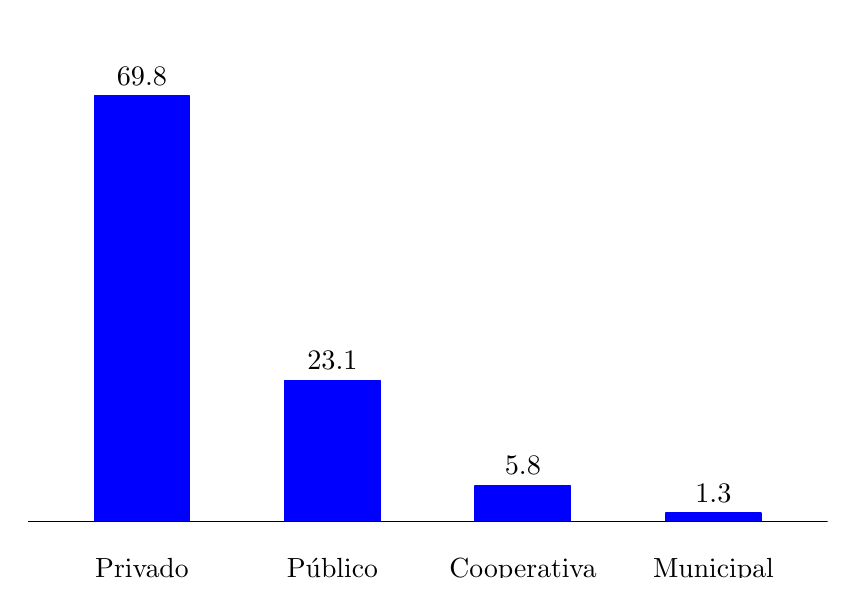
\begin{tikzpicture}[x=1pt,y=1pt]  % Created by tikzDevice version 0.10.1 on 2016-02-29 12:46:52
% !TEX encoding = UTF-8 Unicode
\definecolor{fillColor}{RGB}{255,255,255}
\path[use as bounding box,fill=fillColor,fill opacity=0.00] (0,0) rectangle (289.08,198.74);
\begin{scope}
\path[clip] (  0.00,  0.00) rectangle (289.08,198.74);

\path[] (  0.00,  0.00) rectangle (289.08,198.74);
\end{scope}
\begin{scope}
\path[clip] (  0.00,  0.00) rectangle (289.08,198.74);

\path[] (  0.00, 12.77) rectangle (289.08,181.67);

\path[] ( 41.30, 12.77) --
	( 41.30,181.67);

\path[] (110.13, 12.77) --
	(110.13,181.67);

\path[] (178.95, 12.77) --
	(178.95,181.67);

\path[] (247.78, 12.77) --
	(247.78,181.67);
\definecolor{drawColor}{RGB}{0,0,255}
\definecolor{fillColor}{RGB}{0,0,255}

\path[draw=drawColor,line width= 0.6pt,line join=round,fill=fillColor] ( 24.09, 20.44) rectangle ( 58.50,173.99);

\path[draw=drawColor,line width= 0.6pt,line join=round,fill=fillColor] ( 92.92, 20.44) rectangle (127.33, 71.23);

\path[draw=drawColor,line width= 0.6pt,line join=round,fill=fillColor] (161.75, 20.44) rectangle (196.16, 33.17);

\path[draw=drawColor,line width= 0.6pt,line join=round,fill=fillColor] (230.58, 20.44) rectangle (264.99, 23.26);
\definecolor{drawColor}{RGB}{0,0,0}

\path[draw=drawColor,line width= 0.1pt,line join=round] (  0.00, 20.44) -- (289.08, 20.44);

\node[text=drawColor,anchor=base,inner sep=0pt, outer sep=0pt, scale=  1.02] at ( 41.30,177.96) {69.8};

\node[text=drawColor,anchor=base,inner sep=0pt, outer sep=0pt, scale=  1.02] at (110.13, 75.21) {23.1};

\node[text=drawColor,anchor=base,inner sep=0pt, outer sep=0pt, scale=  1.02] at (178.95, 37.14) {5.8};

\node[text=drawColor,anchor=base,inner sep=0pt, outer sep=0pt, scale=  1.02] at (247.78, 27.24) {1.3};

\path[] (  0.00, 12.77) rectangle (289.08,181.67);
\end{scope}
\begin{scope}
\path[clip] (  0.00,  0.00) rectangle (289.08,198.74);

\path[] (  0.00, 12.77) --
	(289.08, 12.77);
\end{scope}
\begin{scope}
\path[clip] (  0.00,  0.00) rectangle (289.08,198.74);

\path[] ( 41.30, 10.02) --
	( 41.30, 12.77);

\path[] (110.13, 10.02) --
	(110.13, 12.77);

\path[] (178.95, 10.02) --
	(178.95, 12.77);

\path[] (247.78, 10.02) --
	(247.78, 12.77);
\end{scope}
\begin{scope}
\path[clip] (  0.00,  0.00) rectangle (289.08,198.74);
\definecolor{drawColor}{RGB}{0,0,0}

\node[text=drawColor,anchor=base,inner sep=0pt, outer sep=0pt, scale=  1.00] at ( 41.30, -0.00) {Privado};

\node[text=drawColor,anchor=base,inner sep=0pt, outer sep=0pt, scale=  1.00] at (110.13, -0.00) {Público};

\node[text=drawColor,anchor=base,inner sep=0pt, outer sep=0pt, scale=  1.00] at (178.95, -0.00) {Cooperativa};

\node[text=drawColor,anchor=base,inner sep=0pt, outer sep=0pt, scale=  1.00] at (247.78, -0.00) {Municipal};
\end{scope}
  \end{tikzpicture}}{Instituto Nacional de Estadística, con datos del Ministerio de Educación}

\cajita{Inscritos en diversificado e idioma}{En la gráfica  se observa que del total de inscritos en diversificado, 97.4\% reciben clases en idioma español.
	
El 2.6\% de los alumnos de diversificado recibieron clases en algún idioma maya.}{Distribución de inscritos en el ciclo de educación diversificada, según el idioma en el que reciben clases}{República de Guatemala, año 2014, en porcentaje}{\ \\[0mm]\begin{tikzpicture}[x=1pt,y=1pt]  % Created by tikzDevice version 0.7.0 on 2015-08-28 16:54:23
% !TEX encoding = UTF-8 Unicode
\definecolor[named]{fillColor}{rgb}{1.00,1.00,1.00}
\path[use as bounding box,fill=fillColor,fill opacity=0.00] (0,0) rectangle (289.08,198.74);
\begin{scope}
\path[clip] (  0.00,  0.00) rectangle (289.08,198.74);
\definecolor[named]{drawColor}{rgb}{1.00,1.00,1.00}

\path[draw=drawColor,line width= 0.6pt,line join=round,line cap=round] (  0.00,  0.00) rectangle (289.08,198.74);
\end{scope}
\begin{scope}
\path[clip] (  0.00,  0.00) rectangle (289.08,198.74);

\path[] (  7.11, 32.50) rectangle (289.08,174.70);

\path[] ( 34.40, 32.50) --
	( 34.40,174.70);

\path[] ( 79.88, 32.50) --
	( 79.88,174.70);

\path[] (125.36, 32.50) --
	(125.36,174.70);

\path[] (170.84, 32.50) --
	(170.84,174.70);

\path[] (216.31, 32.50) --
	(216.31,174.70);

\path[] (261.79, 32.50) --
	(261.79,174.70);
\definecolor[named]{drawColor}{rgb}{0.00,0.00,1.00}
\definecolor[named]{fillColor}{rgb}{0.00,0.00,1.00}

\path[draw=drawColor,line width= 0.6pt,line join=round,fill=fillColor] ( 16.66, 32.50) rectangle ( 31.67, 36.87);
\definecolor[named]{drawColor}{rgb}{0.62,0.73,1.00}
\definecolor[named]{fillColor}{rgb}{0.62,0.73,1.00}

\path[draw=drawColor,line width= 0.6pt,line join=round,fill=fillColor] ( 37.13, 32.50) rectangle ( 52.14, 33.81);
\definecolor[named]{drawColor}{rgb}{0.00,0.00,1.00}
\definecolor[named]{fillColor}{rgb}{0.00,0.00,1.00}

\path[draw=drawColor,line width= 0.6pt,line join=round,fill=fillColor] ( 62.14, 32.50) rectangle ( 77.15, 54.13);
\definecolor[named]{drawColor}{rgb}{0.62,0.73,1.00}
\definecolor[named]{fillColor}{rgb}{0.62,0.73,1.00}

\path[draw=drawColor,line width= 0.6pt,line join=round,fill=fillColor] ( 82.61, 32.50) rectangle ( 97.62, 63.30);
\definecolor[named]{drawColor}{rgb}{0.00,0.00,1.00}
\definecolor[named]{fillColor}{rgb}{0.00,0.00,1.00}

\path[draw=drawColor,line width= 0.6pt,line join=round,fill=fillColor] (107.62, 32.50) rectangle (122.63, 54.34);
\definecolor[named]{drawColor}{rgb}{0.62,0.73,1.00}
\definecolor[named]{fillColor}{rgb}{0.62,0.73,1.00}

\path[draw=drawColor,line width= 0.6pt,line join=round,fill=fillColor] (128.09, 32.50) rectangle (143.09, 48.01);
\definecolor[named]{drawColor}{rgb}{0.00,0.00,1.00}
\definecolor[named]{fillColor}{rgb}{0.00,0.00,1.00}

\path[draw=drawColor,line width= 0.6pt,line join=round,fill=fillColor] (153.10, 32.50) rectangle (168.11, 35.34);
\definecolor[named]{drawColor}{rgb}{0.62,0.73,1.00}
\definecolor[named]{fillColor}{rgb}{0.62,0.73,1.00}

\path[draw=drawColor,line width= 0.6pt,line join=round,fill=fillColor] (173.56, 32.50) rectangle (188.57, 32.50);
\definecolor[named]{drawColor}{rgb}{0.00,0.00,1.00}
\definecolor[named]{fillColor}{rgb}{0.00,0.00,1.00}

\path[draw=drawColor,line width= 0.6pt,line join=round,fill=fillColor] (198.58, 32.50) rectangle (213.59,138.44);
\definecolor[named]{drawColor}{rgb}{0.62,0.73,1.00}
\definecolor[named]{fillColor}{rgb}{0.62,0.73,1.00}

\path[draw=drawColor,line width= 0.6pt,line join=round,fill=fillColor] (219.04, 32.50) rectangle (234.05,174.70);
\definecolor[named]{drawColor}{rgb}{0.00,0.00,1.00}
\definecolor[named]{fillColor}{rgb}{0.00,0.00,1.00}

\path[draw=drawColor,line width= 0.6pt,line join=round,fill=fillColor] (244.06, 32.50) rectangle (259.06, 94.32);
\definecolor[named]{drawColor}{rgb}{0.62,0.73,1.00}
\definecolor[named]{fillColor}{rgb}{0.62,0.73,1.00}

\path[draw=drawColor,line width= 0.6pt,line join=round,fill=fillColor] (264.52, 32.50) rectangle (279.53, 61.12);
\definecolor[named]{drawColor}{rgb}{0.00,0.00,0.00}
\definecolor[named]{fillColor}{rgb}{0.00,0.00,0.00}

\path[draw=drawColor,line width= 0.6pt,line join=round,fill=fillColor] (  7.11, 32.50) -- (289.08, 32.50);

\node[text=drawColor,anchor=base,inner sep=0pt, outer sep=0pt, scale=  0.82] at ( 24.17, 40.09) {2.0};

\node[text=drawColor,anchor=base,inner sep=0pt, outer sep=0pt, scale=  0.82] at ( 44.63, 37.03) {0.6};

\node[text=drawColor,anchor=base,inner sep=0pt, outer sep=0pt, scale=  0.82] at ( 69.65, 57.35) {9.9};

\node[text=drawColor,anchor=base,inner sep=0pt, outer sep=0pt, scale=  0.82] at ( 90.11, 66.52) {14.1};

\node[text=drawColor,anchor=base,inner sep=0pt, outer sep=0pt, scale=  0.82] at (115.12, 57.57) {10.0};

\node[text=drawColor,anchor=base,inner sep=0pt, outer sep=0pt, scale=  0.82] at (135.59, 51.23) {7.1};

\node[text=drawColor,anchor=base,inner sep=0pt, outer sep=0pt, scale=  0.82] at (160.60, 38.56) {1.3};

\node[text=drawColor,anchor=base,inner sep=0pt, outer sep=0pt, scale=  0.82] at (181.07, 35.72) {0.0};

\node[text=drawColor,anchor=base,inner sep=0pt, outer sep=0pt, scale=  0.82] at (206.08,141.67) {48.5};

\node[text=drawColor,anchor=base,inner sep=0pt, outer sep=0pt, scale=  0.82] at (226.55,177.93) {65.1};

\node[text=drawColor,anchor=base,inner sep=0pt, outer sep=0pt, scale=  0.82] at (251.56, 97.54) {28.3};

\node[text=drawColor,anchor=base,inner sep=0pt, outer sep=0pt, scale=  0.82] at (272.03, 64.34) {13.1};
\end{scope}
\begin{scope}
\path[clip] (  0.00,  0.00) rectangle (289.08,198.74);

\path[] (  7.11, 32.50) --
	(  7.11,174.70);
\end{scope}
\begin{scope}
\path[clip] (  0.00,  0.00) rectangle (289.08,198.74);

\path[] (  7.11, 32.50) --
	(289.08, 32.50);
\end{scope}
\begin{scope}
\path[clip] (  0.00,  0.00) rectangle (289.08,198.74);

\path[] ( 34.40, 28.23) --
	( 34.40, 32.50);

\path[] ( 79.88, 28.23) --
	( 79.88, 32.50);

\path[] (125.36, 28.23) --
	(125.36, 32.50);

\path[] (170.84, 28.23) --
	(170.84, 32.50);

\path[] (216.31, 28.23) --
	(216.31, 32.50);

\path[] (261.79, 28.23) --
	(261.79, 32.50);
\end{scope}
\begin{scope}
\path[clip] (  0.00,  0.00) rectangle (289.08,198.74);
\definecolor[named]{drawColor}{rgb}{0.00,0.00,0.00}

\node[text=drawColor,anchor=base,inner sep=0pt, outer sep=0pt, scale=  1.00] at ( 34.40, 17.57) {Ciencias};

\node[text=drawColor,anchor=base,inner sep=0pt, outer sep=0pt, scale=  1.00] at ( 34.40,  5.69) { naturales};

\node[text=drawColor,anchor=base,inner sep=0pt, outer sep=0pt, scale=  1.00] at ( 79.88, 17.57) {Ingenier\'ias};

\node[text=drawColor,anchor=base,inner sep=0pt, outer sep=0pt, scale=  1.00] at ( 79.88,  5.69) { y tecnolog\'ia};

\node[text=drawColor,anchor=base,inner sep=0pt, outer sep=0pt, scale=  1.00] at (125.36, 17.57) {Ciencias};

\node[text=drawColor,anchor=base,inner sep=0pt, outer sep=0pt, scale=  1.00] at (125.36,  5.69) { m\'edicas};

\node[text=drawColor,anchor=base,inner sep=0pt, outer sep=0pt, scale=  1.00] at (170.84, 17.57) {Ciencias};

\node[text=drawColor,anchor=base,inner sep=0pt, outer sep=0pt, scale=  1.00] at (170.84,  5.69) { agr\'icolas};

\node[text=drawColor,anchor=base,inner sep=0pt, outer sep=0pt, scale=  1.00] at (216.31, 17.57) {Ciencias};

\node[text=drawColor,anchor=base,inner sep=0pt, outer sep=0pt, scale=  1.00] at (216.31,  5.69) { sociales};

\node[text=drawColor,anchor=base,inner sep=0pt, outer sep=0pt, scale=  1.00] at (261.79, 11.63) {Humanidades};
\end{scope}
\coordinate (apoyo) at (57.37,191.07);
\coordinate (longitudFicticia) at (7.11,7.67);
\coordinate (longitud) at (7.11,7.11);
\coordinate (desX) at (138.52,0);
\coordinate (desY) at (0,0.28);
\definecolor[named]{ct1}{HTML}{
0000FF
}
\definecolor[named]{ct2}{HTML}{
9DBBFF
}
\definecolor[named]{ctb1}{HTML}{
0000FF
}
\definecolor[named]{ctb2}{HTML}{
9DBBFF
}
\path [fill=none] (apoyo) rectangle ($(apoyo)+(longitudFicticia)$)
node [xshift=0.3cm,inner sep=0pt, outer sep=0pt,midway,right,scale = 0.9]{P\'ublico};
\draw [color = ctb1,fill=ct1] ( $(apoyo)  + (desY) $) rectangle ($(apoyo)+ (desY) +(longitud)$);
\path [fill=none] ($(apoyo)+(desX)$) rectangle ($(apoyo)+(desX)+(longitudFicticia)$)
node [xshift=0.3cm,inner sep=0pt, outer sep=0pt,midway,right,scale = 0.9]{Privado};
\draw [color = ctb2 ,fill=ct2] ( $(apoyo)  + (desY) + (desX) $) rectangle ($(apoyo)+ (desY)+ (desX) +(longitud)$);
  \end{tikzpicture}}{Instituto Nacional de Estadística, con datos del Ministerio de Educación}

\cajota{Inscritos en diversificado en los departamentos}{El mapa muestra en color celeste los departamentos con la menor cantidad de alumnos inscritos en diversificado fueron: Zacapa 5,820, El Progreso 5,352 y  Totonicapán 4,524.
	
	 Los departamentos con la mayor cantidad de alumnos inscritos en diversificado fueron: Guatemala 126,103, Quetzaltenango 30,631 y San Marcos 24,451.}{Número de inscritos en el ciclo de educación diversificada}{Por departamento, año 2014, en datos absolutos}{\includegraphics[width=52\cuadri]{graficas/diversificado/1_7.pdf} }{Instituto Nacional de Estadística, con datos del Ministerio de Educación}




\INEchaptercarta[Indicadores de educación diversificada]{Indicadores\\ de educación diversificada}{}


\cajita{Cobertura bruta}{La tasa bruta de cobertura en diversificado establece una relación entre la inscripción inicial total sin distinción de edad.
	
	En el año 2009 fue de 33.4\% en el año 2014 fue de 38.0\%, lo cual fue un aumento de 4.7 puntos porcentuales.}{Tasa bruta de cobertura del ciclo de educación diversificada}{República de Guatemala, serie histórica, en porcentaje}{\ \\[0mm]\begin{tikzpicture}[x=1pt,y=1pt]  % Created by tikzDevice version 0.7.0 on 2015-08-31 18:31:43
% !TEX encoding = UTF-8 Unicode
\definecolor[named]{fillColor}{rgb}{1.00,1.00,1.00}
\path[use as bounding box,fill=fillColor,fill opacity=0.00] (0,0) rectangle (289.08,198.74);
\begin{scope}
\path[clip] (  0.00,  0.00) rectangle (289.08,198.74);
\definecolor[named]{drawColor}{rgb}{1.00,1.00,1.00}

\path[draw=drawColor,line width= 0.6pt,line join=round,line cap=round] (  0.00,  0.00) rectangle (289.08,198.74);
\end{scope}
\begin{scope}
\path[clip] (  0.00,  0.00) rectangle (289.08,198.74);

\path[] (  1.64, 17.78) rectangle (280.54,191.48);

\path[] (  1.64, 37.03) --
	(280.54, 37.03);

\path[] (  1.64, 82.48) --
	(280.54, 82.48);

\path[] (  1.64,127.92) --
	(280.54,127.92);

\path[] (  1.64,173.36) --
	(280.54,173.36);

\path[] (  1.64, 59.75) --
	(280.54, 59.75);

\path[] (  1.64,105.20) --
	(280.54,105.20);

\path[] (  1.64,150.64) --
	(280.54,150.64);

\path[] ( 33.83, 17.78) --
	( 33.83,191.48);

\path[] ( 87.46, 17.78) --
	( 87.46,191.48);

\path[] (141.09, 17.78) --
	(141.09,191.48);

\path[] (194.73, 17.78) --
	(194.73,191.48);

\path[] (248.36, 17.78) --
	(248.36,191.48);
\definecolor[named]{drawColor}{rgb}{0.00,0.00,1.00}

\path[draw=drawColor,line width= 1.7pt,line join=round] ( 33.83,121.10) --
	( 87.46,158.59) --
	(141.09,172.23) --
	(194.73,183.59) --
	(248.36,181.32);
\definecolor[named]{drawColor}{rgb}{0.00,0.00,0.00}

\node[text=drawColor,anchor=base,inner sep=0pt, outer sep=0pt, scale=  1.01] at ( 33.83,109.23) {33.4};

\node[text=drawColor,anchor=base east,inner sep=0pt, outer sep=0pt, scale=  1.01] at ( 84.34,158.59) {36.7};

\node[text=drawColor,anchor=base east,inner sep=0pt, outer sep=0pt, scale=  1.01] at (137.98,172.23) {37.9};

\node[text=drawColor,anchor=base,inner sep=0pt, outer sep=0pt, scale=  1.01] at (194.73,187.54) {38.9};

\node[text=drawColor,anchor=base,inner sep=0pt, outer sep=0pt, scale=  1.01] at (248.36,169.44) {38.7};
\definecolor[named]{fillColor}{rgb}{0.00,0.00,0.00}

\path[draw=drawColor,line width= 0.1pt,line join=round,fill=fillColor] (  1.64, 25.67) -- (280.54, 25.67);
\end{scope}
\begin{scope}
\path[clip] (  0.00,  0.00) rectangle (289.08,198.74);

\path[] (  1.64, 17.78) --
	(  1.64,191.48);
\end{scope}
\begin{scope}
\path[clip] (  0.00,  0.00) rectangle (289.08,198.74);

\path[] (  0.00, 59.75) --
	(  1.64, 59.75);

\path[] (  0.00,105.20) --
	(  1.64,105.20);

\path[] (  0.00,150.64) --
	(  1.64,150.64);
\end{scope}
\begin{scope}
\path[clip] (  0.00,  0.00) rectangle (289.08,198.74);

\path[] (  1.64, 17.78) --
	(280.54, 17.78);
\end{scope}
\begin{scope}
\path[clip] (  0.00,  0.00) rectangle (289.08,198.74);

\path[] ( 33.83, 13.51) --
	( 33.83, 17.78);

\path[] ( 87.46, 13.51) --
	( 87.46, 17.78);

\path[] (141.09, 13.51) --
	(141.09, 17.78);

\path[] (194.73, 13.51) --
	(194.73, 17.78);

\path[] (248.36, 13.51) --
	(248.36, 17.78);
\end{scope}
\begin{scope}
\path[clip] (  0.00,  0.00) rectangle (289.08,198.74);
\definecolor[named]{drawColor}{rgb}{0.00,0.00,0.00}

\node[text=drawColor,anchor=base,inner sep=0pt, outer sep=0pt, scale=  1.00] at ( 33.83,  2.85) {2009};

\node[text=drawColor,anchor=base,inner sep=0pt, outer sep=0pt, scale=  1.00] at ( 87.46,  2.85) {2010};

\node[text=drawColor,anchor=base,inner sep=0pt, outer sep=0pt, scale=  1.00] at (141.09,  2.85) {2011};

\node[text=drawColor,anchor=base,inner sep=0pt, outer sep=0pt, scale=  1.00] at (194.73,  2.85) {2012};

\node[text=drawColor,anchor=base,inner sep=0pt, outer sep=0pt, scale=  1.00] at (248.36,  2.85) {2014};
\end{scope}
  \end{tikzpicture}}{Instituto Nacional de Estadística, con datos del Ministerio de Educación}

\cajita{Cobertura bruta por sexo}{La tasa bruta de cobertura en diversificado por sexo fue del 37.7\% para hombres y 38.3\% para mujeres.}{Tasa bruta de cobertura del ciclo de educación diversificada, por sexo}{República de Guatemala, año 2014, en porcentaje}{\ \\[0mm]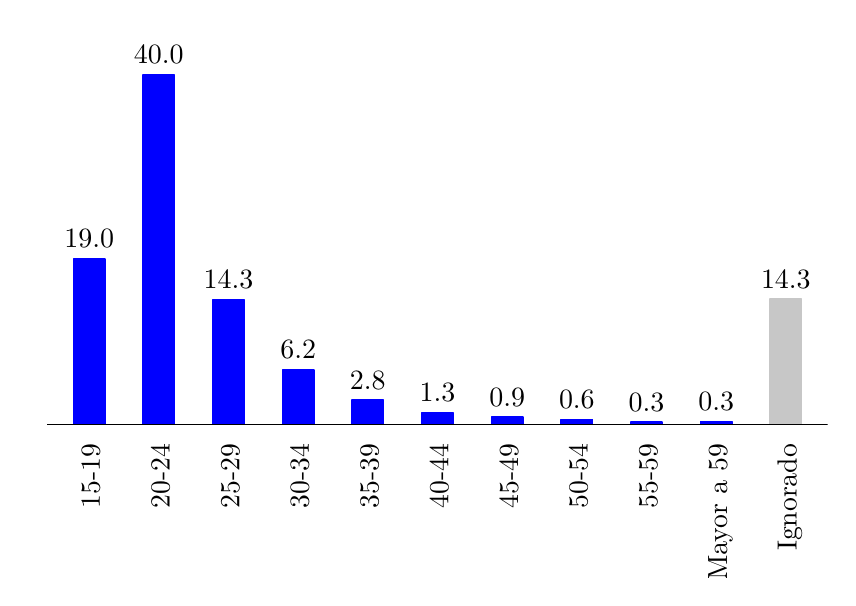
\begin{tikzpicture}[x=1pt,y=1pt]  % Created by tikzDevice version 0.7.0 on 2015-08-28 16:20:10
% !TEX encoding = UTF-8 Unicode
\definecolor[named]{fillColor}{rgb}{1.00,1.00,1.00}
\path[use as bounding box,fill=fillColor,fill opacity=0.00] (0,0) rectangle (289.08,198.74);
\begin{scope}
\path[clip] (  0.00,  0.00) rectangle (289.08,198.74);
\definecolor[named]{drawColor}{rgb}{1.00,1.00,1.00}

\path[draw=drawColor,line width= 0.6pt,line join=round,line cap=round] (  0.00,  0.00) rectangle (289.08,198.74);
\end{scope}
\begin{scope}
\path[clip] (  0.00,  0.00) rectangle (289.08,198.74);

\path[] (  7.11, 55.39) rectangle (289.08,181.67);

\path[] ( 22.22, 55.39) --
	( 22.22,181.67);

\path[] ( 47.39, 55.39) --
	( 47.39,181.67);

\path[] ( 72.57, 55.39) --
	( 72.57,181.67);

\path[] ( 97.75, 55.39) --
	( 97.75,181.67);

\path[] (122.92, 55.39) --
	(122.92,181.67);

\path[] (148.10, 55.39) --
	(148.10,181.67);

\path[] (173.27, 55.39) --
	(173.27,181.67);

\path[] (198.45, 55.39) --
	(198.45,181.67);

\path[] (223.62, 55.39) --
	(223.62,181.67);

\path[] (248.80, 55.39) --
	(248.80,181.67);

\path[] (273.97, 55.39) --
	(273.97,181.67);
\definecolor[named]{drawColor}{rgb}{0.00,0.00,1.00}
\definecolor[named]{fillColor}{rgb}{0.00,0.00,1.00}

\path[draw=drawColor,line width= 0.6pt,line join=round,fill=fillColor] ( 16.55, 55.39) rectangle ( 27.88,115.21);

\path[draw=drawColor,line width= 0.6pt,line join=round,fill=fillColor] ( 41.73, 55.39) rectangle ( 53.06,181.67);

\path[draw=drawColor,line width= 0.6pt,line join=round,fill=fillColor] ( 66.91, 55.39) rectangle ( 78.23,100.50);

\path[draw=drawColor,line width= 0.6pt,line join=round,fill=fillColor] ( 92.08, 55.39) rectangle (103.41, 75.09);

\path[draw=drawColor,line width= 0.6pt,line join=round,fill=fillColor] (117.26, 55.39) rectangle (128.59, 64.15);

\path[draw=drawColor,line width= 0.6pt,line join=round,fill=fillColor] (142.43, 55.39) rectangle (153.76, 59.63);

\path[draw=drawColor,line width= 0.6pt,line join=round,fill=fillColor] (167.61, 55.39) rectangle (178.94, 58.08);

\path[draw=drawColor,line width= 0.6pt,line join=round,fill=fillColor] (192.78, 55.39) rectangle (204.11, 57.21);

\path[draw=drawColor,line width= 0.6pt,line join=round,fill=fillColor] (217.96, 55.39) rectangle (229.29, 56.24);

\path[draw=drawColor,line width= 0.6pt,line join=round,fill=fillColor] (243.13, 55.39) rectangle (254.46, 56.41);
\definecolor[named]{drawColor}{rgb}{0.78,0.78,0.78}
\definecolor[named]{fillColor}{rgb}{0.78,0.78,0.78}

\path[draw=drawColor,line width= 0.6pt,line join=round,fill=fillColor] (268.31, 55.39) rectangle (279.64,100.63);
\definecolor[named]{drawColor}{rgb}{0.00,0.00,0.00}
\definecolor[named]{fillColor}{rgb}{0.00,0.00,0.00}

\path[draw=drawColor,line width= 0.1pt,line join=round,fill=fillColor] (  7.11, 55.39) -- (289.08, 55.39);

\node[text=drawColor,anchor=base,inner sep=0pt, outer sep=0pt, scale=  1.01] at ( 22.22,119.17) {19.0};

\node[text=drawColor,anchor=base,inner sep=0pt, outer sep=0pt, scale=  1.01] at ( 47.39,185.63) {40.0};

\node[text=drawColor,anchor=base,inner sep=0pt, outer sep=0pt, scale=  1.01] at ( 72.57,104.45) {14.3};

\node[text=drawColor,anchor=base,inner sep=0pt, outer sep=0pt, scale=  1.01] at ( 97.75, 79.04) {6.2};

\node[text=drawColor,anchor=base,inner sep=0pt, outer sep=0pt, scale=  1.01] at (122.92, 68.10) {2.8};

\node[text=drawColor,anchor=base,inner sep=0pt, outer sep=0pt, scale=  1.01] at (148.10, 63.59) {1.3};

\node[text=drawColor,anchor=base,inner sep=0pt, outer sep=0pt, scale=  1.01] at (173.27, 62.03) {0.9};

\node[text=drawColor,anchor=base,inner sep=0pt, outer sep=0pt, scale=  1.01] at (198.45, 61.17) {0.6};

\node[text=drawColor,anchor=base,inner sep=0pt, outer sep=0pt, scale=  1.01] at (223.62, 60.20) {0.3};

\node[text=drawColor,anchor=base,inner sep=0pt, outer sep=0pt, scale=  1.01] at (248.80, 60.37) {0.3};

\node[text=drawColor,anchor=base,inner sep=0pt, outer sep=0pt, scale=  1.01] at (273.97,104.59) {14.3};
\end{scope}
\begin{scope}
\path[clip] (  0.00,  0.00) rectangle (289.08,198.74);

\path[] (  7.11, 55.39) --
	(  7.11,181.67);
\end{scope}
\begin{scope}
\path[clip] (  0.00,  0.00) rectangle (289.08,198.74);

\path[] (  7.11, 55.39) --
	(289.08, 55.39);
\end{scope}
\begin{scope}
\path[clip] (  0.00,  0.00) rectangle (289.08,198.74);

\path[] ( 22.22, 51.12) --
	( 22.22, 55.39);

\path[] ( 47.39, 51.12) --
	( 47.39, 55.39);

\path[] ( 72.57, 51.12) --
	( 72.57, 55.39);

\path[] ( 97.75, 51.12) --
	( 97.75, 55.39);

\path[] (122.92, 51.12) --
	(122.92, 55.39);

\path[] (148.10, 51.12) --
	(148.10, 55.39);

\path[] (173.27, 51.12) --
	(173.27, 55.39);

\path[] (198.45, 51.12) --
	(198.45, 55.39);

\path[] (223.62, 51.12) --
	(223.62, 55.39);

\path[] (248.80, 51.12) --
	(248.80, 55.39);

\path[] (273.97, 51.12) --
	(273.97, 55.39);
\end{scope}
\begin{scope}
\path[clip] (  0.00,  0.00) rectangle (289.08,198.74);
\definecolor[named]{drawColor}{rgb}{0.00,0.00,0.00}

\node[text=drawColor,rotate= 90.00,anchor=base east,inner sep=0pt, outer sep=0pt, scale=  1.00] at ( 26.13, 48.28) {15-19};

\node[text=drawColor,rotate= 90.00,anchor=base east,inner sep=0pt, outer sep=0pt, scale=  1.00] at ( 51.30, 48.28) {20-24};

\node[text=drawColor,rotate= 90.00,anchor=base east,inner sep=0pt, outer sep=0pt, scale=  1.00] at ( 76.48, 48.28) {25-29};

\node[text=drawColor,rotate= 90.00,anchor=base east,inner sep=0pt, outer sep=0pt, scale=  1.00] at (101.65, 48.28) {30-34};

\node[text=drawColor,rotate= 90.00,anchor=base east,inner sep=0pt, outer sep=0pt, scale=  1.00] at (126.83, 48.28) {35-39};

\node[text=drawColor,rotate= 90.00,anchor=base east,inner sep=0pt, outer sep=0pt, scale=  1.00] at (152.01, 48.28) {40-44};

\node[text=drawColor,rotate= 90.00,anchor=base east,inner sep=0pt, outer sep=0pt, scale=  1.00] at (177.18, 48.28) {45-49};

\node[text=drawColor,rotate= 90.00,anchor=base east,inner sep=0pt, outer sep=0pt, scale=  1.00] at (202.36, 48.28) {50-54};

\node[text=drawColor,rotate= 90.00,anchor=base east,inner sep=0pt, outer sep=0pt, scale=  1.00] at (227.53, 48.28) {55-59};

\node[text=drawColor,rotate= 90.00,anchor=base east,inner sep=0pt, outer sep=0pt, scale=  1.00] at (252.71, 48.28) {Mayor a  59};

\node[text=drawColor,rotate= 90.00,anchor=base east,inner sep=0pt, outer sep=0pt, scale=  1.00] at (277.88, 48.28) {Ignorado};
\end{scope}
  \end{tikzpicture}}{Instituto Nacional de Estadística, con datos del Ministerio de Educación}

\cajota{Cobertura bruta en los departamentos}{Los departamentos con las menores tasas brutas de cobertura en diversificado en el 2014 fueron: Huehuetenango 21.6\%, Alta Verapaz 19.2\% y Totonicapán 15.0\%.
	
	 Los departamentos con las mayores tasas brutas de cobertura en diversificado: Guatemala 62.5\%, Quetzaltenango 57.0\% y  Retalhuleu 49.6\%.}{Tasa bruta de cobertura del ciclo de educación diversificada}{Por departamento, año 2014, en porcentaje}{\includegraphics[width=52\cuadri]{graficas/diversificado/1_10.pdf} }{Instituto Nacional de Estadística, con datos del Ministerio de Educación}

\cajita{Cobertura neta}{La tasa neta de cobertura en diversificado es la relación que existe entre la parte de la inscripción inicial que se encuentra en la edad escolar de 16 a 19 años y la población en edad escolar de 16 a 19 años.
	
	En el año 2009 el 21.2\% de cobertura y en el 2014 fue de 24.4\% el cual fue un aumento en 3.2 puntos porcentuales.}{Tasa neta de cobertura del ciclo de educación diversificada}{República de Guatemala, serie histórica, en porcentaje}{\ \\[0mm]\begin{tikzpicture}[x=1pt,y=1pt]  % Created by tikzDevice version 0.10.1 on 2016-02-29 12:47:47
% !TEX encoding = UTF-8 Unicode
\definecolor{fillColor}{RGB}{255,255,255}
\path[use as bounding box,fill=fillColor,fill opacity=0.00] (0,0) rectangle (289.08,198.74);
\begin{scope}
\path[clip] (  0.00,  0.00) rectangle (289.08,198.74);

\path[] (  0.00,  0.00) rectangle (289.08,198.74);
\end{scope}
\begin{scope}
\path[clip] (  0.00,  0.00) rectangle (289.08,198.74);

\path[] ( -0.52, 15.61) rectangle (280.54,191.48);

\path[] (  0.00, 51.17) --
	(280.54, 51.17);

\path[] (  0.00,106.30) --
	(280.54,106.30);

\path[] (  0.00,161.44) --
	(280.54,161.44);

\path[] (  0.00, 23.61) --
	(280.54, 23.61);

\path[] (  0.00, 78.74) --
	(280.54, 78.74);

\path[] (  0.00,133.87) --
	(280.54,133.87);

\path[] (  0.00,189.00) --
	(280.54,189.00);

\path[] ( 26.68, 15.61) --
	( 26.68,191.48);

\path[] ( 72.01, 15.61) --
	( 72.01,191.48);

\path[] (117.35, 15.61) --
	(117.35,191.48);

\path[] (162.68, 15.61) --
	(162.68,191.48);

\path[] (208.01, 15.61) --
	(208.01,191.48);

\path[] (253.34, 15.61) --
	(253.34,191.48);
\definecolor{drawColor}{RGB}{0,0,255}

\path[draw=drawColor,line width= 1.7pt,line join=round] ( 26.68,147.21) --
	( 72.01,159.56) --
	(117.35,172.35) --
	(162.68,179.74) --
	(208.01,183.49) --
	(253.34,182.17);
\definecolor{drawColor}{RGB}{0,0,0}

\node[text=drawColor,anchor=base,inner sep=0pt, outer sep=0pt, scale=  1.02] at ( 26.68,135.30) {21.2};

\node[text=drawColor,anchor=base east,inner sep=0pt, outer sep=0pt, scale=  1.02] at ( 68.89,159.56) {22.3};

\node[text=drawColor,anchor=base east,inner sep=0pt, outer sep=0pt, scale=  1.02] at (114.22,172.35) {23.5};

\node[text=drawColor,anchor=base east,inner sep=0pt, outer sep=0pt, scale=  1.02] at (159.55,179.74) {24.2};

\node[text=drawColor,anchor=base,inner sep=0pt, outer sep=0pt, scale=  1.02] at (208.01,187.46) {24.5};

\node[text=drawColor,anchor=base,inner sep=0pt, outer sep=0pt, scale=  1.02] at (253.34,170.25) {24.4};

\path[draw=drawColor,line width= 0.1pt,line join=round] (  0.00, 23.61) -- (280.54, 23.61);

\path[] ( -0.52, 15.61) rectangle (280.54,191.48);
\end{scope}
\begin{scope}
\path[clip] (  0.00,  0.00) rectangle (289.08,198.74);

\path[] (  0.00, 15.61) --
	(280.54, 15.61);
\end{scope}
\begin{scope}
\path[clip] (  0.00,  0.00) rectangle (289.08,198.74);

\path[] ( 26.68, 12.86) --
	( 26.68, 15.61);

\path[] ( 72.01, 12.86) --
	( 72.01, 15.61);

\path[] (117.35, 12.86) --
	(117.35, 15.61);

\path[] (162.68, 12.86) --
	(162.68, 15.61);

\path[] (208.01, 12.86) --
	(208.01, 15.61);

\path[] (253.34, 12.86) --
	(253.34, 15.61);
\end{scope}
\begin{scope}
\path[clip] (  0.00,  0.00) rectangle (289.08,198.74);
\definecolor{drawColor}{RGB}{0,0,0}

\node[text=drawColor,anchor=base,inner sep=0pt, outer sep=0pt, scale=  1.00] at ( 26.68,  2.85) {2009};

\node[text=drawColor,anchor=base,inner sep=0pt, outer sep=0pt, scale=  1.00] at ( 72.01,  2.85) {2010};

\node[text=drawColor,anchor=base,inner sep=0pt, outer sep=0pt, scale=  1.00] at (117.35,  2.85) {2011};

\node[text=drawColor,anchor=base,inner sep=0pt, outer sep=0pt, scale=  1.00] at (162.68,  2.85) {2012};

\node[text=drawColor,anchor=base,inner sep=0pt, outer sep=0pt, scale=  1.00] at (208.01,  2.85) {2013};

\node[text=drawColor,anchor=base,inner sep=0pt, outer sep=0pt, scale=  1.00] at (253.34,  2.85) {2014};
\end{scope}
  \end{tikzpicture}}{Instituto Nacional de Estadística, con datos del Ministerio de Educación}

\cajita{Cobertura neta por sexo}{La tasa neta de cobertura en diversificado por sexo fue del 23.8\% para hombres y 24.9\% para las mujeres.}{Tasa neta de cobertura del ciclo de educación diversificada, por sexo}{República de Guatemala, año 2014, en porcentaje}{\ \\[0mm]\begin{tikzpicture}[x=1pt,y=1pt]  % Created by tikzDevice version 0.7.0 on 2015-09-01 14:24:00
% !TEX encoding = UTF-8 Unicode
\definecolor[named]{fillColor}{rgb}{1.00,1.00,1.00}
\path[use as bounding box,fill=fillColor,fill opacity=0.00] (0,0) rectangle (289.08,198.74);
\begin{scope}
\path[clip] (  0.00,  0.00) rectangle (289.08,198.74);
\definecolor[named]{drawColor}{rgb}{1.00,1.00,1.00}

\path[draw=drawColor,line width= 0.6pt,line join=round,line cap=round] (  0.00,  0.00) rectangle (289.08,198.74);
\end{scope}
\begin{scope}
\path[clip] (  0.00,  0.00) rectangle (289.08,198.74);

\path[] (  1.64, 17.78) rectangle (280.54,191.48);

\path[] (  1.64, 47.21) --
	(280.54, 47.21);

\path[] (  1.64, 90.30) --
	(280.54, 90.30);

\path[] (  1.64,133.39) --
	(280.54,133.39);

\path[] (  1.64,176.48) --
	(280.54,176.48);

\path[] (  1.64, 25.67) --
	(280.54, 25.67);

\path[] (  1.64, 68.76) --
	(280.54, 68.76);

\path[] (  1.64,111.85) --
	(280.54,111.85);

\path[] (  1.64,154.93) --
	(280.54,154.93);

\path[] ( 33.83, 17.78) --
	( 33.83,191.48);

\path[] ( 87.46, 17.78) --
	( 87.46,191.48);

\path[] (141.09, 17.78) --
	(141.09,191.48);

\path[] (194.73, 17.78) --
	(194.73,191.48);

\path[] (248.36, 17.78) --
	(248.36,191.48);
\definecolor[named]{drawColor}{rgb}{0.00,0.00,1.00}

\path[draw=drawColor,line width= 1.7pt,line join=round] ( 33.83, 96.77) --
	( 87.46,123.48) --
	(141.09,133.39) --
	(194.73,167.64) --
	(248.36,183.59);
\definecolor[named]{drawColor}{rgb}{0.00,0.00,0.00}

\node[text=drawColor,anchor=base,inner sep=0pt, outer sep=0pt, scale=  1.01] at ( 33.83, 84.90) {53.0};

\node[text=drawColor,anchor=base east,inner sep=0pt, outer sep=0pt, scale=  1.01] at ( 84.34,123.48) {65.4};

\node[text=drawColor,anchor=base east,inner sep=0pt, outer sep=0pt, scale=  1.01] at (137.98,133.39) {70.0};

\node[text=drawColor,anchor=base east,inner sep=0pt, outer sep=0pt, scale=  1.01] at (191.61,167.64) {85.9};

\node[text=drawColor,anchor=base,inner sep=0pt, outer sep=0pt, scale=  1.01] at (248.36,187.54) {93.3};
\definecolor[named]{fillColor}{rgb}{0.00,0.00,0.00}

\path[draw=drawColor,line width= 0.1pt,line join=round,fill=fillColor] (  1.64, 25.67) -- (280.54, 25.67);
\end{scope}
\begin{scope}
\path[clip] (  0.00,  0.00) rectangle (289.08,198.74);

\path[] (  1.64, 17.78) --
	(  1.64,191.48);
\end{scope}
\begin{scope}
\path[clip] (  0.00,  0.00) rectangle (289.08,198.74);

\path[] (  0.00, 25.67) --
	(  1.64, 25.67);

\path[] (  0.00, 68.76) --
	(  1.64, 68.76);

\path[] (  0.00,111.85) --
	(  1.64,111.85);

\path[] (  0.00,154.93) --
	(  1.64,154.93);
\end{scope}
\begin{scope}
\path[clip] (  0.00,  0.00) rectangle (289.08,198.74);

\path[] (  1.64, 17.78) --
	(280.54, 17.78);
\end{scope}
\begin{scope}
\path[clip] (  0.00,  0.00) rectangle (289.08,198.74);

\path[] ( 33.83, 13.51) --
	( 33.83, 17.78);

\path[] ( 87.46, 13.51) --
	( 87.46, 17.78);

\path[] (141.09, 13.51) --
	(141.09, 17.78);

\path[] (194.73, 13.51) --
	(194.73, 17.78);

\path[] (248.36, 13.51) --
	(248.36, 17.78);
\end{scope}
\begin{scope}
\path[clip] (  0.00,  0.00) rectangle (289.08,198.74);
\definecolor[named]{drawColor}{rgb}{0.00,0.00,0.00}

\node[text=drawColor,anchor=base,inner sep=0pt, outer sep=0pt, scale=  1.00] at ( 33.83,  2.85) {1987};

\node[text=drawColor,anchor=base,inner sep=0pt, outer sep=0pt, scale=  1.00] at ( 87.46,  2.85) {1995};

\node[text=drawColor,anchor=base,inner sep=0pt, outer sep=0pt, scale=  1.00] at (141.09,  2.85) {1998/99};

\node[text=drawColor,anchor=base,inner sep=0pt, outer sep=0pt, scale=  1.00] at (194.73,  2.85) {2002};

\node[text=drawColor,anchor=base,inner sep=0pt, outer sep=0pt, scale=  1.00] at (248.36,  2.85) {2008/09};
\end{scope}
  \end{tikzpicture}}{Instituto Nacional de Estadística, con datos del Ministerio de Educación}

\cajota{Cobertura neta en los departamentos}{Los departamentos con las menores tasas netas de cobertura en diversificado en el 2014 fueron: Quiché 12.4\%, Alta Verapaz 10.3\% y Totonicapán 9.2\%.

	 Los departamentos con las más altas tasas netas de cobertura en diversificado fueron:  Guatemala 41.3\%, Quetzaltenango 36.5\% y El Progreso 33.3\%. }{Tasa neta de cobertura del ciclo de educación diversificada}{Por departamento, año 2014, en porcentaje}{\includegraphics[width=52\cuadri]{graficas/diversificado/1_13.pdf} }{Instituto Nacional de Estadística, con datos del Ministerio de Educación}




\cajita{Repitencia}{La tasa de repitencia en diversificado es la relación que existe entre el número de repitentes y el número de alumnos que en el año  estaban inscritos en el mismo grado.
	
	En el año 2009 fue  del 1.2\% y en el año 2014 fue de 0.8\% lo cual representó una disminución en 0.4 puntos porcentuales.}{Tasa de repitencia del ciclo de educación diversificada}{República de Guatemala, serie histórica, en porcentaje}{\ \\[0mm]\begin{tikzpicture}[x=1pt,y=1pt]  % Created by tikzDevice version 0.10.1 on 2016-02-29 12:48:20
% !TEX encoding = UTF-8 Unicode
\definecolor{fillColor}{RGB}{255,255,255}
\path[use as bounding box,fill=fillColor,fill opacity=0.00] (0,0) rectangle (289.08,198.74);
\begin{scope}
\path[clip] (  0.00,  0.00) rectangle (289.08,198.74);

\path[] (  0.00,  0.00) rectangle (289.08,198.74);
\end{scope}
\begin{scope}
\path[clip] (  0.00,  0.00) rectangle (289.08,198.74);

\path[] ( 10.27, 15.61) rectangle (280.54,191.48);

\path[] ( 10.27, 47.68) --
	(280.54, 47.68);

\path[] ( 10.27, 95.84) --
	(280.54, 95.84);

\path[] ( 10.27,144.00) --
	(280.54,144.00);

\path[] ( 10.27, 23.61) --
	(280.54, 23.61);

\path[] ( 10.27, 71.76) --
	(280.54, 71.76);

\path[] ( 10.27,119.92) --
	(280.54,119.92);

\path[] ( 10.27,168.08) --
	(280.54,168.08);

\path[] ( 36.43, 15.61) --
	( 36.43,191.48);

\path[] ( 80.02, 15.61) --
	( 80.02,191.48);

\path[] (123.61, 15.61) --
	(123.61,191.48);

\path[] (167.20, 15.61) --
	(167.20,191.48);

\path[] (210.80, 15.61) --
	(210.80,191.48);

\path[] (254.39, 15.61) --
	(254.39,191.48);
\definecolor{drawColor}{RGB}{0,0,255}

\path[draw=drawColor,line width= 1.7pt,line join=round] ( 36.43,135.33) --
	( 80.02,111.25) --
	(123.61,101.62) --
	(167.20,183.49) --
	(210.80,114.14) --
	(254.39, 98.73);
\definecolor{drawColor}{RGB}{0,0,0}

\node[text=drawColor,anchor=base,inner sep=0pt, outer sep=0pt, scale=  1.02] at ( 36.43,139.30) {1.2};

\node[text=drawColor,anchor=base west,inner sep=0pt, outer sep=0pt, scale=  1.02] at ( 80.02,115.22) {0.9};

\node[text=drawColor,anchor=base,inner sep=0pt, outer sep=0pt, scale=  1.02] at (123.61, 89.71) {0.8};

\node[text=drawColor,anchor=base,inner sep=0pt, outer sep=0pt, scale=  1.02] at (167.20,187.46) {1.7};

\node[text=drawColor,anchor=base west,inner sep=0pt, outer sep=0pt, scale=  1.02] at (210.80,118.11) {0.9};

\node[text=drawColor,anchor=base,inner sep=0pt, outer sep=0pt, scale=  1.02] at (254.39, 86.82) {0.8};

\path[draw=drawColor,line width= 0.1pt,line join=round] ( 10.27, 23.61) -- (280.54, 23.61);

\path[] ( 10.27, 15.61) rectangle (280.54,191.48);
\end{scope}
\begin{scope}
\path[clip] (  0.00,  0.00) rectangle (289.08,198.74);

\path[] ( 10.27, 15.61) --
	( 10.27,191.48);
\end{scope}
\begin{scope}
\path[clip] (  0.00,  0.00) rectangle (289.08,198.74);
\definecolor{drawColor}{RGB}{255,255,255}

\node[text=drawColor,text opacity=0.00,anchor=base east,inner sep=0pt, outer sep=0pt, scale=  1.00] at (  5.32, 19.70) {0.0};

\node[text=drawColor,text opacity=0.00,anchor=base east,inner sep=0pt, outer sep=0pt, scale=  1.00] at (  5.32, 67.86) {0.5};

\node[text=drawColor,text opacity=0.00,anchor=base east,inner sep=0pt, outer sep=0pt, scale=  1.00] at (  5.32,116.01) {1.0};

\node[text=drawColor,text opacity=0.00,anchor=base east,inner sep=0pt, outer sep=0pt, scale=  1.00] at (  5.32,164.17) {1.5};
\end{scope}
\begin{scope}
\path[clip] (  0.00,  0.00) rectangle (289.08,198.74);

\path[] (  7.52, 23.61) --
	( 10.27, 23.61);

\path[] (  7.52, 71.76) --
	( 10.27, 71.76);

\path[] (  7.52,119.92) --
	( 10.27,119.92);

\path[] (  7.52,168.08) --
	( 10.27,168.08);
\end{scope}
\begin{scope}
\path[clip] (  0.00,  0.00) rectangle (289.08,198.74);

\path[] ( 10.27, 15.61) --
	(280.54, 15.61);
\end{scope}
\begin{scope}
\path[clip] (  0.00,  0.00) rectangle (289.08,198.74);

\path[] ( 36.43, 12.86) --
	( 36.43, 15.61);

\path[] ( 80.02, 12.86) --
	( 80.02, 15.61);

\path[] (123.61, 12.86) --
	(123.61, 15.61);

\path[] (167.20, 12.86) --
	(167.20, 15.61);

\path[] (210.80, 12.86) --
	(210.80, 15.61);

\path[] (254.39, 12.86) --
	(254.39, 15.61);
\end{scope}
\begin{scope}
\path[clip] (  0.00,  0.00) rectangle (289.08,198.74);
\definecolor{drawColor}{RGB}{0,0,0}

\node[text=drawColor,anchor=base,inner sep=0pt, outer sep=0pt, scale=  1.00] at ( 36.43,  2.85) {2009};

\node[text=drawColor,anchor=base,inner sep=0pt, outer sep=0pt, scale=  1.00] at ( 80.02,  2.85) {2010};

\node[text=drawColor,anchor=base,inner sep=0pt, outer sep=0pt, scale=  1.00] at (123.61,  2.85) {2011};

\node[text=drawColor,anchor=base,inner sep=0pt, outer sep=0pt, scale=  1.00] at (167.20,  2.85) {2012};

\node[text=drawColor,anchor=base,inner sep=0pt, outer sep=0pt, scale=  1.00] at (210.80,  2.85) {2013};

\node[text=drawColor,anchor=base,inner sep=0pt, outer sep=0pt, scale=  1.00] at (254.39,  2.85) {2014};
\end{scope}
  \end{tikzpicture}}{Instituto Nacional de Estadística, con datos del Ministerio de Educación}

\cajita{Repitencia por sexo}{La tasa de repitencia en diversificado por sexo fue del 0.9\% para hombres y 0.7\% para las mujeres. }{Tasa de repitencia del ciclo de educación diversificada, por sexo}{República de Guatemala, año 2014, en porcentaje}{\ \\[0mm]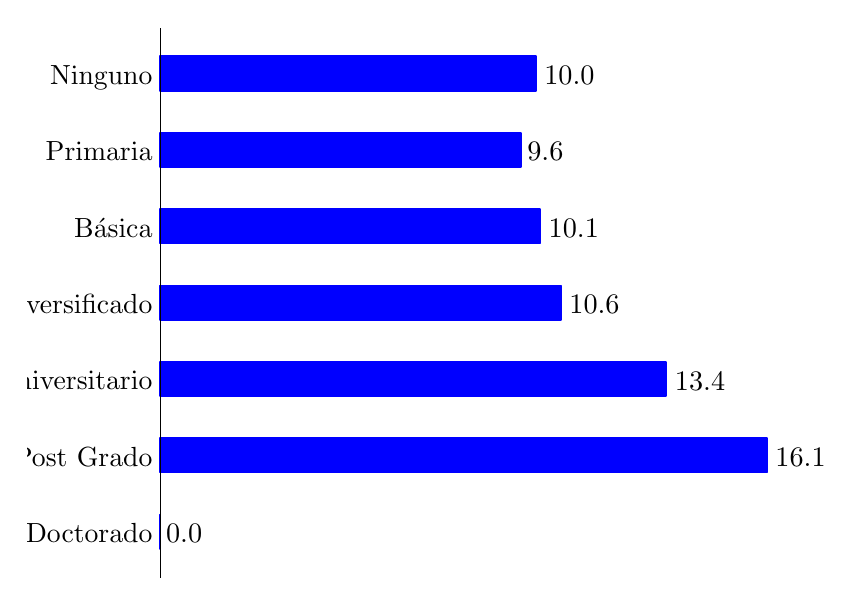
\begin{tikzpicture}[x=1pt,y=1pt]  % Created by tikzDevice version 0.10.1 on 2016-02-29 14:42:48
% !TEX encoding = UTF-8 Unicode
\definecolor{fillColor}{RGB}{255,255,255}
\path[use as bounding box,fill=fillColor,fill opacity=0.00] (0,0) rectangle (289.08,198.74);
\begin{scope}
\path[clip] (  0.00,  0.00) rectangle (289.08,198.74);

\path[] (  0.00,  0.00) rectangle (289.08,198.74);
\end{scope}
\begin{scope}
\path[clip] (  0.00,  0.00) rectangle (289.08,198.74);

\path[] ( 47.80,  0.00) rectangle (267.09,198.74);

\path[] ( 47.80, 16.56) --
	(267.09, 16.56);

\path[] ( 47.80, 44.16) --
	(267.09, 44.16);

\path[] ( 47.80, 71.77) --
	(267.09, 71.77);

\path[] ( 47.80, 99.37) --
	(267.09, 99.37);

\path[] ( 47.80,126.97) --
	(267.09,126.97);

\path[] ( 47.80,154.58) --
	(267.09,154.58);

\path[] ( 47.80,182.18) --
	(267.09,182.18);
\definecolor{drawColor}{RGB}{0,0,255}
\definecolor{fillColor}{RGB}{0,0,255}

\path[draw=drawColor,line width= 0.6pt,line join=round,fill=fillColor] ( 47.80, 10.35) rectangle ( 47.80, 22.77);

\path[draw=drawColor,line width= 0.6pt,line join=round,fill=fillColor] ( 47.80, 37.95) rectangle (267.09, 50.38);

\path[draw=drawColor,line width= 0.6pt,line join=round,fill=fillColor] ( 47.80, 65.56) rectangle (230.77, 77.98);

\path[draw=drawColor,line width= 0.6pt,line join=round,fill=fillColor] ( 47.80, 93.16) rectangle (192.63,105.58);

\path[draw=drawColor,line width= 0.6pt,line join=round,fill=fillColor] ( 47.80,120.76) rectangle (185.14,133.19);

\path[draw=drawColor,line width= 0.6pt,line join=round,fill=fillColor] ( 47.80,148.37) rectangle (178.32,160.79);

\path[draw=drawColor,line width= 0.6pt,line join=round,fill=fillColor] ( 47.80,175.97) rectangle (183.58,188.39);
\definecolor{drawColor}{RGB}{0,0,0}

\path[draw=drawColor,line width= 0.1pt,line join=round] ( 47.80,  0.00) -- ( 47.80,198.74);

\node[text=drawColor,anchor=base west,inner sep=0pt, outer sep=0pt, scale=  1.02] at ( 50.03, 12.59) {0.0};

\node[text=drawColor,anchor=base west,inner sep=0pt, outer sep=0pt, scale=  1.02] at (270.21, 40.19) {16.1};

\node[text=drawColor,anchor=base west,inner sep=0pt, outer sep=0pt, scale=  1.02] at (233.89, 67.80) {13.4};

\node[text=drawColor,anchor=base west,inner sep=0pt, outer sep=0pt, scale=  1.02] at (195.76, 95.40) {10.6};

\node[text=drawColor,anchor=base west,inner sep=0pt, outer sep=0pt, scale=  1.02] at (188.27,123.00) {10.1};

\node[text=drawColor,anchor=base west,inner sep=0pt, outer sep=0pt, scale=  1.02] at (180.56,150.61) {9.6};

\node[text=drawColor,anchor=base west,inner sep=0pt, outer sep=0pt, scale=  1.02] at (186.71,178.21) {10.0};

\path[] ( 47.80,  0.00) rectangle (267.09,198.74);
\end{scope}
\begin{scope}
\path[clip] (  0.00,  0.00) rectangle (289.08,198.74);

\path[] ( 47.80,  0.00) --
	( 47.80,198.74);
\end{scope}
\begin{scope}
\path[clip] (  0.00,  0.00) rectangle (289.08,198.74);
\definecolor{drawColor}{RGB}{0,0,0}

\node[text=drawColor,anchor=base east,inner sep=0pt, outer sep=0pt, scale=  1.00] at ( 45.05, 12.65) {Doctorado};

\node[text=drawColor,anchor=base east,inner sep=0pt, outer sep=0pt, scale=  1.00] at ( 45.05, 40.26) {Post Grado};

\node[text=drawColor,anchor=base east,inner sep=0pt, outer sep=0pt, scale=  1.00] at ( 45.05, 67.86) {Universitario};

\node[text=drawColor,anchor=base east,inner sep=0pt, outer sep=0pt, scale=  1.00] at ( 45.05, 95.46) {Diversificado};

\node[text=drawColor,anchor=base east,inner sep=0pt, outer sep=0pt, scale=  1.00] at ( 45.05,123.07) {Básica};

\node[text=drawColor,anchor=base east,inner sep=0pt, outer sep=0pt, scale=  1.00] at ( 45.05,150.67) {Primaria};

\node[text=drawColor,anchor=base east,inner sep=0pt, outer sep=0pt, scale=  1.00] at ( 45.05,178.27) {Ninguno};
\end{scope}
\begin{scope}
\path[clip] (  0.00,  0.00) rectangle (289.08,198.74);

\path[] ( 45.05, 16.56) --
	( 47.80, 16.56);

\path[] ( 45.05, 44.16) --
	( 47.80, 44.16);

\path[] ( 45.05, 71.77) --
	( 47.80, 71.77);

\path[] ( 45.05, 99.37) --
	( 47.80, 99.37);

\path[] ( 45.05,126.97) --
	( 47.80,126.97);

\path[] ( 45.05,154.58) --
	( 47.80,154.58);

\path[] ( 45.05,182.18) --
	( 47.80,182.18);
\end{scope}
  \end{tikzpicture}}{Instituto Nacional de Estadística, con datos del Ministerio de Educación}

\cajota{Repitencia en los departamentos}{El mapa muestra en color celeste los departamentos con las menores tasas de repitencia en diversificado fueron: Suchitepéquez 0.3\%, Jutiapa 0.3\%  y Petén 0.2\%.
	
	 Los departamentos con las más  altas tasa de repitencia en diversificado en el 2014 fueron: Zacapa 1.4\%, Alta Verapaz 1.2\% y Totonicapán 1.2\%. El departamento de Guatemala presentó una tasa de repitencia de 1.0\%.}{Tasa de repitencia del ciclo de educación diversificada}{Por departamento, año 2014, en porcentaje}{\includegraphics[width=52\cuadri]{graficas/diversificado/1_16.pdf} }{Instituto Nacional de Estadística, con datos del Ministerio de Educación}






\cajita{Sobre-edad}{La tasa de sobre-edad en diversificado es la relación que existe entre la cantidad de alumnos inscritos en los diferentes grados de un nivel educativo, con dos o más años de atraso escolar por encima de la edad correspondiente al grado de estudio.
	
	En el año 2009 fue de 31.3\% y en el 2014 fue 26.6\%, una disminución en 4.7 puntos porcentuales.}{Tasa de sobre-edad del ciclo de educación diversificada}{República de Guatemala, serie histórica, en porcentaje}{\ \\[0mm]\begin{tikzpicture}[x=1pt,y=1pt]  % Created by tikzDevice version 0.10.1 on 2016-02-29 12:48:35
% !TEX encoding = UTF-8 Unicode
\definecolor{fillColor}{RGB}{255,255,255}
\path[use as bounding box,fill=fillColor,fill opacity=0.00] (0,0) rectangle (289.08,198.74);
\begin{scope}
\path[clip] (  0.00,  0.00) rectangle (289.08,198.74);

\path[] (  0.00,  0.00) rectangle (289.08,198.74);
\end{scope}
\begin{scope}
\path[clip] (  0.00,  0.00) rectangle (289.08,198.74);

\path[] (  6.12, 15.61) rectangle (280.54,191.48);

\path[] (  6.12, 41.28) --
	(280.54, 41.28);

\path[] (  6.12, 76.62) --
	(280.54, 76.62);

\path[] (  6.12,111.96) --
	(280.54,111.96);

\path[] (  6.12,147.30) --
	(280.54,147.30);

\path[] (  6.12,182.64) --
	(280.54,182.64);

\path[] (  6.12, 23.61) --
	(280.54, 23.61);

\path[] (  6.12, 58.95) --
	(280.54, 58.95);

\path[] (  6.12, 94.29) --
	(280.54, 94.29);

\path[] (  6.12,129.63) --
	(280.54,129.63);

\path[] (  6.12,164.97) --
	(280.54,164.97);

\path[] ( 32.67, 15.61) --
	( 32.67,191.48);

\path[] ( 76.94, 15.61) --
	( 76.94,191.48);

\path[] (121.20, 15.61) --
	(121.20,191.48);

\path[] (165.46, 15.61) --
	(165.46,191.48);

\path[] (209.72, 15.61) --
	(209.72,191.48);

\path[] (253.99, 15.61) --
	(253.99,191.48);
\definecolor{drawColor}{RGB}{0,0,255}

\path[draw=drawColor,line width= 1.7pt,line join=round] ( 32.67,183.49) --
	( 76.94,171.90) --
	(121.20,162.71) --
	(165.46,162.99) --
	(209.72,142.63) --
	(253.99,117.19);
\definecolor{drawColor}{RGB}{0,0,0}

\node[text=drawColor,anchor=base,inner sep=0pt, outer sep=0pt, scale=  1.02] at ( 32.67,187.46) {31.3};

\node[text=drawColor,anchor=base west,inner sep=0pt, outer sep=0pt, scale=  1.02] at ( 76.94,175.87) {30.5};

\node[text=drawColor,anchor=base,inner sep=0pt, outer sep=0pt, scale=  1.02] at (121.20,150.80) {29.8};

\node[text=drawColor,anchor=base,inner sep=0pt, outer sep=0pt, scale=  1.02] at (165.46,166.96) {29.9};

\node[text=drawColor,anchor=base west,inner sep=0pt, outer sep=0pt, scale=  1.02] at (209.72,146.61) {28.4};

\node[text=drawColor,anchor=base,inner sep=0pt, outer sep=0pt, scale=  1.02] at (253.99,105.28) {26.6};

\path[draw=drawColor,line width= 0.1pt,line join=round] (  6.12, 23.61) -- (280.54, 23.61);

\path[] (  6.12, 15.61) rectangle (280.54,191.48);
\end{scope}
\begin{scope}
\path[clip] (  0.00,  0.00) rectangle (289.08,198.74);

\path[] (  6.12, 15.61) --
	(  6.12,191.48);
\end{scope}
\begin{scope}
\path[clip] (  0.00,  0.00) rectangle (289.08,198.74);
\definecolor{drawColor}{RGB}{255,255,255}

\node[text=drawColor,text opacity=0.00,anchor=base east,inner sep=0pt, outer sep=0pt, scale=  1.00] at (  1.17, 19.70) {20.0};

\node[text=drawColor,text opacity=0.00,anchor=base east,inner sep=0pt, outer sep=0pt, scale=  1.00] at (  1.17, 55.04) {22.5};

\node[text=drawColor,text opacity=0.00,anchor=base east,inner sep=0pt, outer sep=0pt, scale=  1.00] at (  1.17, 90.38) {25.0};

\node[text=drawColor,text opacity=0.00,anchor=base east,inner sep=0pt, outer sep=0pt, scale=  1.00] at (  1.17,125.72) {27.5};

\node[text=drawColor,text opacity=0.00,anchor=base east,inner sep=0pt, outer sep=0pt, scale=  1.00] at (  1.17,161.06) {30.0};
\end{scope}
\begin{scope}
\path[clip] (  0.00,  0.00) rectangle (289.08,198.74);

\path[] (  3.37, 23.61) --
	(  6.12, 23.61);

\path[] (  3.37, 58.95) --
	(  6.12, 58.95);

\path[] (  3.37, 94.29) --
	(  6.12, 94.29);

\path[] (  3.37,129.63) --
	(  6.12,129.63);

\path[] (  3.37,164.97) --
	(  6.12,164.97);
\end{scope}
\begin{scope}
\path[clip] (  0.00,  0.00) rectangle (289.08,198.74);

\path[] (  6.12, 15.61) --
	(280.54, 15.61);
\end{scope}
\begin{scope}
\path[clip] (  0.00,  0.00) rectangle (289.08,198.74);

\path[] ( 32.67, 12.86) --
	( 32.67, 15.61);

\path[] ( 76.94, 12.86) --
	( 76.94, 15.61);

\path[] (121.20, 12.86) --
	(121.20, 15.61);

\path[] (165.46, 12.86) --
	(165.46, 15.61);

\path[] (209.72, 12.86) --
	(209.72, 15.61);

\path[] (253.99, 12.86) --
	(253.99, 15.61);
\end{scope}
\begin{scope}
\path[clip] (  0.00,  0.00) rectangle (289.08,198.74);
\definecolor{drawColor}{RGB}{0,0,0}

\node[text=drawColor,anchor=base,inner sep=0pt, outer sep=0pt, scale=  1.00] at ( 32.67,  2.85) {2009};

\node[text=drawColor,anchor=base,inner sep=0pt, outer sep=0pt, scale=  1.00] at ( 76.94,  2.85) {2010};

\node[text=drawColor,anchor=base,inner sep=0pt, outer sep=0pt, scale=  1.00] at (121.20,  2.85) {2011};

\node[text=drawColor,anchor=base,inner sep=0pt, outer sep=0pt, scale=  1.00] at (165.46,  2.85) {2012};

\node[text=drawColor,anchor=base,inner sep=0pt, outer sep=0pt, scale=  1.00] at (209.72,  2.85) {2013};

\node[text=drawColor,anchor=base,inner sep=0pt, outer sep=0pt, scale=  1.00] at (253.99,  2.85) {2014};
\end{scope}
  \end{tikzpicture}}{Instituto Nacional de Estadística, con datos del Ministerio de Educación}

\cajita{Sobre-edad por sexo}{La tasa de sobre-edad en diversificado por sexo fue 28.9\% para hombres y 24.3\% para mujeres.}{Tasa de sobre-edad del ciclo de educación diversificada, por sexo}{República de Guatemala, año 2014, en porcentaje}{\ \\[0mm]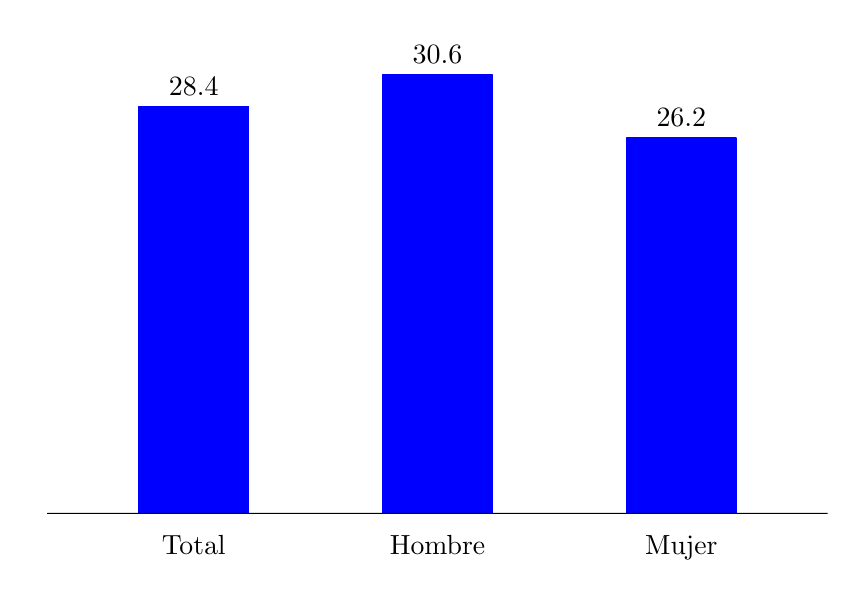
\begin{tikzpicture}[x=1pt,y=1pt]  % Created by tikzDevice version 0.7.0 on 2015-08-28 13:12:27
% !TEX encoding = UTF-8 Unicode
\definecolor[named]{fillColor}{rgb}{1.00,1.00,1.00}
\path[use as bounding box,fill=fillColor,fill opacity=0.00] (0,0) rectangle (289.08,198.74);
\begin{scope}
\path[clip] (  0.00,  0.00) rectangle (289.08,198.74);
\definecolor[named]{drawColor}{rgb}{1.00,1.00,1.00}

\path[draw=drawColor,line width= 0.6pt,line join=round,line cap=round] (  0.00,  0.00) rectangle (289.08,198.74);
\end{scope}
\begin{scope}
\path[clip] (  0.00,  0.00) rectangle (289.08,198.74);

\path[] (  7.11, 23.47) rectangle (289.08,181.67);

\path[] ( 59.98, 23.47) --
	( 59.98,181.67);

\path[] (148.10, 23.47) --
	(148.10,181.67);

\path[] (236.21, 23.47) --
	(236.21,181.67);
\definecolor[named]{drawColor}{rgb}{0.00,0.00,1.00}
\definecolor[named]{fillColor}{rgb}{0.00,0.00,1.00}

\path[draw=drawColor,line width= 0.6pt,line join=round,fill=fillColor] ( 40.16, 23.47) rectangle ( 79.81,170.30);

\path[draw=drawColor,line width= 0.6pt,line join=round,fill=fillColor] (128.27, 23.47) rectangle (167.92,181.67);

\path[draw=drawColor,line width= 0.6pt,line join=round,fill=fillColor] (216.39, 23.47) rectangle (256.04,158.92);
\definecolor[named]{drawColor}{rgb}{0.00,0.00,0.00}
\definecolor[named]{fillColor}{rgb}{0.00,0.00,0.00}

\path[draw=drawColor,line width= 0.1pt,line join=round,fill=fillColor] (  7.11, 23.47) -- (289.08, 23.47);

\node[text=drawColor,anchor=base,inner sep=0pt, outer sep=0pt, scale=  1.01] at ( 59.98,174.25) {28.4};

\node[text=drawColor,anchor=base,inner sep=0pt, outer sep=0pt, scale=  1.01] at (148.10,185.63) {30.6};

\node[text=drawColor,anchor=base,inner sep=0pt, outer sep=0pt, scale=  1.01] at (236.21,162.88) {26.2};
\end{scope}
\begin{scope}
\path[clip] (  0.00,  0.00) rectangle (289.08,198.74);

\path[] (  7.11, 23.47) --
	(  7.11,181.67);
\end{scope}
\begin{scope}
\path[clip] (  0.00,  0.00) rectangle (289.08,198.74);

\path[] (  7.11, 23.47) --
	(289.08, 23.47);
\end{scope}
\begin{scope}
\path[clip] (  0.00,  0.00) rectangle (289.08,198.74);

\path[] ( 59.98, 19.20) --
	( 59.98, 23.47);

\path[] (148.10, 19.20) --
	(148.10, 23.47);

\path[] (236.21, 19.20) --
	(236.21, 23.47);
\end{scope}
\begin{scope}
\path[clip] (  0.00,  0.00) rectangle (289.08,198.74);
\definecolor[named]{drawColor}{rgb}{0.00,0.00,0.00}

\node[text=drawColor,anchor=base,inner sep=0pt, outer sep=0pt, scale=  1.00] at ( 59.98,  8.54) {Total};

\node[text=drawColor,anchor=base,inner sep=0pt, outer sep=0pt, scale=  1.00] at (148.10,  8.54) {Hombre};

\node[text=drawColor,anchor=base,inner sep=0pt, outer sep=0pt, scale=  1.00] at (236.21,  8.54) {Mujer};
\end{scope}
  \end{tikzpicture}}{Instituto Nacional de Estadística, con datos del Ministerio de Educación}

\cajota{Sobre-edad en los departamentos}{El mapa muestra en color celeste los departamentos con las menores tasas de sobre-edad en diversificado: Quetzaltenango 22.2\%, El Progreso 21.5\% y Zacapa 19.6\%.
	
	 Los departamentos que en el 2014 tuvieron las más altas tasas  de sobre-edad en diversificado: Alta Verapaz 39.7\%, Quiché 35.2\% y Petén 30.4\%. En el departamento de Guatemala, la tasa de sobre-edad fue de 26.7\%. }{Tasa de sobre-edad del ciclo de educación diversificada}{Por departamento, año 2014, en porcentaje}{\includegraphics[width=52\cuadri]{graficas/diversificado/1_19.pdf} }{Instituto Nacional de Estadística, con datos del Ministerio de Educación}





\cajita{Deserción}{La tasa de deserción en diversificado se refiere a la cantidad de alumnos que no concluyen el ciclo lectivo.
	
	Presentó en el año 2009 el 6.5\% y en el año 2014 fue de 1.5\%, disminución en 5.0 puntos porcentuales.}{Tasa de deserción del ciclo de educación diversificada}{República de Guatemala, serie histórica, en porcentaje}{\ \\[0mm]\begin{tikzpicture}[x=1pt,y=1pt]  % Created by tikzDevice version 0.7.0 on 2015-08-31 18:35:32
% !TEX encoding = UTF-8 Unicode
\definecolor[named]{fillColor}{rgb}{1.00,1.00,1.00}
\path[use as bounding box,fill=fillColor,fill opacity=0.00] (0,0) rectangle (289.08,198.74);
\begin{scope}
\path[clip] (  0.00,  0.00) rectangle (289.08,198.74);
\definecolor[named]{drawColor}{rgb}{1.00,1.00,1.00}

\path[draw=drawColor,line width= 0.6pt,line join=round,line cap=round] (  0.00,  0.00) rectangle (289.08,198.74);
\end{scope}
\begin{scope}
\path[clip] (  0.00,  0.00) rectangle (289.08,198.74);

\path[] (  1.64, 17.78) rectangle (280.54,191.48);

\path[] (  1.64, 48.89) --
	(280.54, 48.89);

\path[] (  1.64, 95.34) --
	(280.54, 95.34);

\path[] (  1.64,141.79) --
	(280.54,141.79);

\path[] (  1.64,188.23) --
	(280.54,188.23);

\path[] (  1.64, 25.67) --
	(280.54, 25.67);

\path[] (  1.64, 72.12) --
	(280.54, 72.12);

\path[] (  1.64,118.56) --
	(280.54,118.56);

\path[] (  1.64,165.01) --
	(280.54,165.01);

\path[] ( 33.83, 17.78) --
	( 33.83,191.48);

\path[] ( 87.46, 17.78) --
	( 87.46,191.48);

\path[] (141.09, 17.78) --
	(141.09,191.48);

\path[] (194.73, 17.78) --
	(194.73,191.48);

\path[] (248.36, 17.78) --
	(248.36,191.48);
\definecolor[named]{drawColor}{rgb}{0.00,0.00,1.00}

\path[draw=drawColor,line width= 1.7pt,line join=round] ( 33.83,132.50) --
	( 87.46,183.59) --
	(141.09,114.85) --
	(194.73,103.70) --
	(248.36, 89.77);
\definecolor[named]{drawColor}{rgb}{0.00,0.00,0.00}

\node[text=drawColor,anchor=base,inner sep=0pt, outer sep=0pt, scale=  1.01] at ( 33.83,120.63) {6.5};

\node[text=drawColor,anchor=base,inner sep=0pt, outer sep=0pt, scale=  1.01] at ( 87.46,187.54) {12.0};

\node[text=drawColor,anchor=base west,inner sep=0pt, outer sep=0pt, scale=  1.01] at (141.09,118.80) {4.6};

\node[text=drawColor,anchor=base west,inner sep=0pt, outer sep=0pt, scale=  1.01] at (194.73,107.66) {3.4};

\node[text=drawColor,anchor=base,inner sep=0pt, outer sep=0pt, scale=  1.01] at (248.36, 77.90) {1.9};
\definecolor[named]{fillColor}{rgb}{0.00,0.00,0.00}

\path[draw=drawColor,line width= 0.1pt,line join=round,fill=fillColor] (  1.64, 25.67) -- (280.54, 25.67);
\end{scope}
\begin{scope}
\path[clip] (  0.00,  0.00) rectangle (289.08,198.74);

\path[] (  1.64, 17.78) --
	(  1.64,191.48);
\end{scope}
\begin{scope}
\path[clip] (  0.00,  0.00) rectangle (289.08,198.74);

\path[] (  0.00, 25.67) --
	(  1.64, 25.67);

\path[] (  0.00, 72.12) --
	(  1.64, 72.12);

\path[] (  0.00,118.56) --
	(  1.64,118.56);

\path[] (  0.00,165.01) --
	(  1.64,165.01);
\end{scope}
\begin{scope}
\path[clip] (  0.00,  0.00) rectangle (289.08,198.74);

\path[] (  1.64, 17.78) --
	(280.54, 17.78);
\end{scope}
\begin{scope}
\path[clip] (  0.00,  0.00) rectangle (289.08,198.74);

\path[] ( 33.83, 13.51) --
	( 33.83, 17.78);

\path[] ( 87.46, 13.51) --
	( 87.46, 17.78);

\path[] (141.09, 13.51) --
	(141.09, 17.78);

\path[] (194.73, 13.51) --
	(194.73, 17.78);

\path[] (248.36, 13.51) --
	(248.36, 17.78);
\end{scope}
\begin{scope}
\path[clip] (  0.00,  0.00) rectangle (289.08,198.74);
\definecolor[named]{drawColor}{rgb}{0.00,0.00,0.00}

\node[text=drawColor,anchor=base,inner sep=0pt, outer sep=0pt, scale=  1.00] at ( 33.83,  2.85) {2009};

\node[text=drawColor,anchor=base,inner sep=0pt, outer sep=0pt, scale=  1.00] at ( 87.46,  2.85) {2010};

\node[text=drawColor,anchor=base,inner sep=0pt, outer sep=0pt, scale=  1.00] at (141.09,  2.85) {2011};

\node[text=drawColor,anchor=base,inner sep=0pt, outer sep=0pt, scale=  1.00] at (194.73,  2.85) {2012};

\node[text=drawColor,anchor=base,inner sep=0pt, outer sep=0pt, scale=  1.00] at (248.36,  2.85) {2014};
\end{scope}
  \end{tikzpicture}}{Instituto Nacional de Estadística, con datos del Ministerio de Educación}

\cajita{Deserción por sexo}{La tasa de deserción en diversificado por sexo fue del 2.3\% para hombres y 0.7\% para las mujeres.}{Tasa de deserción del ciclo de educación diversificada, por sexo}{República de Guatemala, año 2014, en porcentaje}{\ \\[0mm]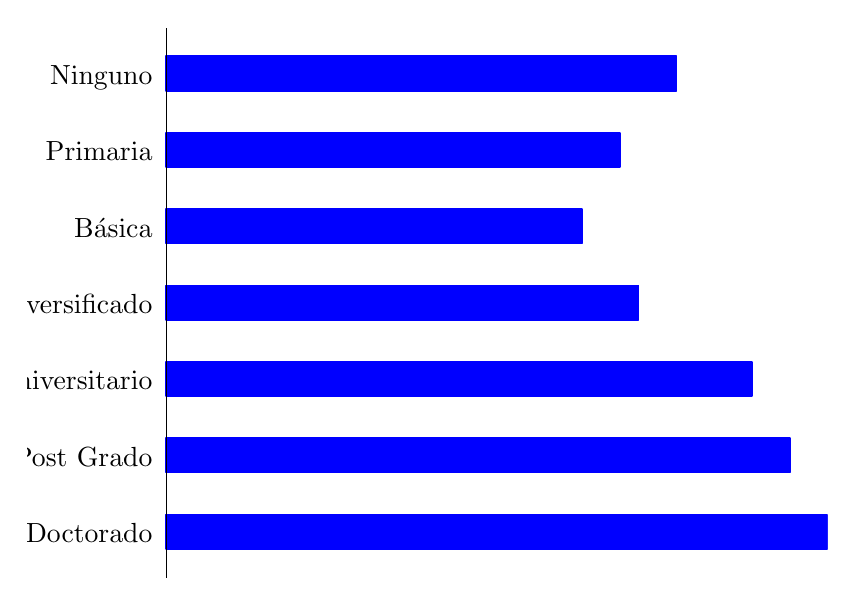
\begin{tikzpicture}[x=1pt,y=1pt]  % Created by tikzDevice version 0.10.1 on 2016-02-29 14:47:24
% !TEX encoding = UTF-8 Unicode
\definecolor{fillColor}{RGB}{255,255,255}
\path[use as bounding box,fill=fillColor,fill opacity=0.00] (0,0) rectangle (289.08,198.74);
\begin{scope}
\path[clip] (  0.00,  0.00) rectangle (289.08,198.74);

\path[] (  0.00,  0.00) rectangle (289.08,198.74);
\end{scope}
\begin{scope}
\path[clip] (  0.00,  0.00) rectangle (289.08,198.74);

\path[] ( 50.00,  0.00) rectangle (289.08,198.74);

\path[] ( 50.00, 16.56) --
	(289.08, 16.56);

\path[] ( 50.00, 44.16) --
	(289.08, 44.16);

\path[] ( 50.00, 71.77) --
	(289.08, 71.77);

\path[] ( 50.00, 99.37) --
	(289.08, 99.37);

\path[] ( 50.00,126.97) --
	(289.08,126.97);

\path[] ( 50.00,154.58) --
	(289.08,154.58);

\path[] ( 50.00,182.18) --
	(289.08,182.18);
\definecolor{drawColor}{RGB}{0,0,255}
\definecolor{fillColor}{RGB}{0,0,255}

\path[draw=drawColor,line width= 0.6pt,line join=round,fill=fillColor] ( 50.00, 10.35) rectangle (289.08, 22.77);

\path[draw=drawColor,line width= 0.6pt,line join=round,fill=fillColor] ( 50.00, 37.95) rectangle (275.42, 50.38);

\path[draw=drawColor,line width= 0.6pt,line join=round,fill=fillColor] ( 50.00, 65.56) rectangle (261.76, 77.98);

\path[draw=drawColor,line width= 0.6pt,line join=round,fill=fillColor] ( 50.00, 93.16) rectangle (220.77,105.58);

\path[draw=drawColor,line width= 0.6pt,line join=round,fill=fillColor] ( 50.00,120.76) rectangle (200.28,133.19);

\path[draw=drawColor,line width= 0.6pt,line join=round,fill=fillColor] ( 50.00,148.37) rectangle (213.94,160.79);

\path[draw=drawColor,line width= 0.6pt,line join=round,fill=fillColor] ( 50.00,175.97) rectangle (234.43,188.39);
\definecolor{drawColor}{RGB}{0,0,0}

\path[draw=drawColor,line width= 0.1pt,line join=round] ( 50.00,  0.00) -- ( 50.00,198.74);

\path[] ( 50.00,  0.00) rectangle (289.08,198.74);
\end{scope}
\begin{scope}
\path[clip] (  0.00,  0.00) rectangle (289.08,198.74);

\path[] ( 50.00,  0.00) --
	( 50.00,198.74);
\end{scope}
\begin{scope}
\path[clip] (  0.00,  0.00) rectangle (289.08,198.74);
\definecolor{drawColor}{RGB}{0,0,0}

\node[text=drawColor,anchor=base east,inner sep=0pt, outer sep=0pt, scale=  1.00] at ( 45.05, 12.65) {Doctorado};

\node[text=drawColor,anchor=base east,inner sep=0pt, outer sep=0pt, scale=  1.00] at ( 45.05, 40.26) {Post Grado};

\node[text=drawColor,anchor=base east,inner sep=0pt, outer sep=0pt, scale=  1.00] at ( 45.05, 67.86) {Universitario};

\node[text=drawColor,anchor=base east,inner sep=0pt, outer sep=0pt, scale=  1.00] at ( 45.05, 95.46) {Diversificado};

\node[text=drawColor,anchor=base east,inner sep=0pt, outer sep=0pt, scale=  1.00] at ( 45.05,123.07) {Básica};

\node[text=drawColor,anchor=base east,inner sep=0pt, outer sep=0pt, scale=  1.00] at ( 45.05,150.67) {Primaria};

\node[text=drawColor,anchor=base east,inner sep=0pt, outer sep=0pt, scale=  1.00] at ( 45.05,178.27) {Ninguno};
\end{scope}
\begin{scope}
\path[clip] (  0.00,  0.00) rectangle (289.08,198.74);

\path[] ( 47.25, 16.56) --
	( 50.00, 16.56);

\path[] ( 47.25, 44.16) --
	( 50.00, 44.16);

\path[] ( 47.25, 71.77) --
	( 50.00, 71.77);

\path[] ( 47.25, 99.37) --
	( 50.00, 99.37);

\path[] ( 47.25,126.97) --
	( 50.00,126.97);

\path[] ( 47.25,154.58) --
	( 50.00,154.58);

\path[] ( 47.25,182.18) --
	( 50.00,182.18);
\end{scope}
  \end{tikzpicture}}{Instituto Nacional de Estadística, con datos del Ministerio de Educación}

\cajota{Deserción en los departamentos}{Los departamentos donde hubo alta tasa de deserción en diversificado fueron: San Marcos 3.78\%, Zacapa 3.76\% y Sololá 3.49\%. En el departamento de Guatemala la tasa de deserción fue de 0.26\%.	}{Tasa de deserción del ciclo de educación diversificada}{Por departamento, año 2014, en porcentaje}{\includegraphics[width=52\cuadri]{graficas/diversificado/1_22.pdf} }{Instituto Nacional de Estadística, con datos del Ministerio de Educación}




\cajita{Aprobación}{La tasa de aprobación en diversificado se refiere a la cantidad de alumnos que culminaron y aprobaron el ciclo lectivo.
	
	Presentó el año 2009 el 76\% y en el  2014 fue de 83.1\%, aumento en 7.1 puntos porcentuales.}{Tasa de aprobación del ciclo de educación diversificada}{República de Guatemala, serie histórica, en porcentaje}{\ \\[0mm]\begin{tikzpicture}[x=1pt,y=1pt]  % Created by tikzDevice version 0.10.1 on 2016-02-29 12:49:38
% !TEX encoding = UTF-8 Unicode
\definecolor{fillColor}{RGB}{255,255,255}
\path[use as bounding box,fill=fillColor,fill opacity=0.00] (0,0) rectangle (289.08,198.74);
\begin{scope}
\path[clip] (  0.00,  0.00) rectangle (289.08,198.74);

\path[] (  0.00,  0.00) rectangle (289.08,198.74);
\end{scope}
\begin{scope}
\path[clip] (  0.00,  0.00) rectangle (289.08,198.74);

\path[] ( -0.52, 15.61) rectangle (280.54,191.48);

\path[] (  0.00, 40.92) --
	(280.54, 40.92);

\path[] (  0.00, 75.54) --
	(280.54, 75.54);

\path[] (  0.00,110.16) --
	(280.54,110.16);

\path[] (  0.00,144.78) --
	(280.54,144.78);

\path[] (  0.00,179.40) --
	(280.54,179.40);

\path[] (  0.00, 23.61) --
	(280.54, 23.61);

\path[] (  0.00, 58.23) --
	(280.54, 58.23);

\path[] (  0.00, 92.85) --
	(280.54, 92.85);

\path[] (  0.00,127.47) --
	(280.54,127.47);

\path[] (  0.00,162.09) --
	(280.54,162.09);

\path[] ( 26.68, 15.61) --
	( 26.68,191.48);

\path[] ( 72.01, 15.61) --
	( 72.01,191.48);

\path[] (117.35, 15.61) --
	(117.35,191.48);

\path[] (162.68, 15.61) --
	(162.68,191.48);

\path[] (208.01, 15.61) --
	(208.01,191.48);

\path[] (253.34, 15.61) --
	(253.34,191.48);
\definecolor{drawColor}{RGB}{0,0,255}

\path[draw=drawColor,line width= 1.7pt,line join=round] ( 26.68,134.40) --
	( 72.01,123.04) --
	(117.35,130.52) --
	(162.68,143.67) --
	(208.01,162.58) --
	(253.34,183.49);
\definecolor{drawColor}{RGB}{0,0,0}

\node[text=drawColor,anchor=base,inner sep=0pt, outer sep=0pt, scale=  1.02] at ( 26.68,138.37) {76.0};

\node[text=drawColor,anchor=base,inner sep=0pt, outer sep=0pt, scale=  1.02] at ( 72.01,111.13) {74.4};

\node[text=drawColor,anchor=base east,inner sep=0pt, outer sep=0pt, scale=  1.02] at (114.22,130.52) {75.4};

\node[text=drawColor,anchor=base east,inner sep=0pt, outer sep=0pt, scale=  1.02] at (159.55,143.67) {77.3};

\node[text=drawColor,anchor=base east,inner sep=0pt, outer sep=0pt, scale=  1.02] at (204.88,162.58) {80.1};

\node[text=drawColor,anchor=base,inner sep=0pt, outer sep=0pt, scale=  1.02] at (253.34,187.46) {83.1};

\path[draw=drawColor,line width= 0.1pt,line join=round] (  0.00, 23.61) -- (280.54, 23.61);

\path[] ( -0.52, 15.61) rectangle (280.54,191.48);
\end{scope}
\begin{scope}
\path[clip] (  0.00,  0.00) rectangle (289.08,198.74);

\path[] (  0.00, 15.61) --
	(280.54, 15.61);
\end{scope}
\begin{scope}
\path[clip] (  0.00,  0.00) rectangle (289.08,198.74);

\path[] ( 26.68, 12.86) --
	( 26.68, 15.61);

\path[] ( 72.01, 12.86) --
	( 72.01, 15.61);

\path[] (117.35, 12.86) --
	(117.35, 15.61);

\path[] (162.68, 12.86) --
	(162.68, 15.61);

\path[] (208.01, 12.86) --
	(208.01, 15.61);

\path[] (253.34, 12.86) --
	(253.34, 15.61);
\end{scope}
\begin{scope}
\path[clip] (  0.00,  0.00) rectangle (289.08,198.74);
\definecolor{drawColor}{RGB}{0,0,0}

\node[text=drawColor,anchor=base,inner sep=0pt, outer sep=0pt, scale=  1.00] at ( 26.68,  2.85) {2009};

\node[text=drawColor,anchor=base,inner sep=0pt, outer sep=0pt, scale=  1.00] at ( 72.01,  2.85) {2010};

\node[text=drawColor,anchor=base,inner sep=0pt, outer sep=0pt, scale=  1.00] at (117.35,  2.85) {2011};

\node[text=drawColor,anchor=base,inner sep=0pt, outer sep=0pt, scale=  1.00] at (162.68,  2.85) {2012};

\node[text=drawColor,anchor=base,inner sep=0pt, outer sep=0pt, scale=  1.00] at (208.01,  2.85) {2013};

\node[text=drawColor,anchor=base,inner sep=0pt, outer sep=0pt, scale=  1.00] at (253.34,  2.85) {2014};
\end{scope}
  \end{tikzpicture}}{Instituto Nacional de Estadística, con datos del Ministerio de Educación}

\cajita{Aprobación por sexo}{La tasa de aprobación en diversificado por sexo fue del 80.2\% para hombres y 85.8\% para las mujeres.}{Tasa de aprobación del ciclo de educación diversificada, por sexo}{República de Guatemala, año 2014, en porcentaje}{\ \\[0mm]\begin{tikzpicture}[x=1pt,y=1pt]  \input{graficas/diversificado/1_24.tex}  \end{tikzpicture}}{Instituto Nacional de Estadística, con datos del Ministerio de Educación}

\cajota{Aprobación en los departamentos}{El mapa muestra en color celeste los departamentos con las menores tasas de aprobación en diversificado en el 2013 fueron:  Quetzaltenango 80.7\%, San Marcos 80.3\% y Alta Verapaz 75.6\%.
	
	 Los departamentos con las mayores tasas de aprobación en diversificado fueron: Huehuetenango 88.5\%, Chiquimula 87.0\% y Jutiapa 86.5\%. El departamento de Guatemala presentó una tasa de aprobación de 82.8\%.}{Tasa de aprobación del ciclo de educación diversificada}{Por departamento, año 2014, en porcentaje}{\includegraphics[width=52\cuadri]{graficas/diversificado/1_25.pdf} }{Instituto Nacional de Estadística, con datos del Ministerio de Educación}



